%==== Document Setup (usthesis)======================================
\documentclass[report,                       %... Document type
               12pt,oneside,openany,a4paper, %... Layout
               goldenblock,                      %... A5 type block(default changed to goldenblock)
               afrikaans,english,         %... Afrikaans default language
               ]{usthesis}

%
% PLEASE read the USthesis documentation for the class options
% and how to set line and paragraph spacing
%

%==== Language setup ================================================
 \usepackage[latin1]{inputenc}%................... Recognizes �, �, etc
 \usepackage{babel}%.............................. Language setup

%==== Math setup ====================================================
 \usepackage{amsmath}%............................ Advanced math (before fonts)
 \renewcommand{\vec}[1]{\boldsymbol{\mathbf{#1}}}
 \usepackage{amssymb}%............................ AMS Symbol fonts

%==== Font setup (default is Computer Modern) =======================
 \usepackage[T1]{fontenc}%........................ Type 1 fonts
 \usepackage{textcomp}%........................... Additional text character
 \usepackage{bm}%................................. Bold math symbols (after fonts)
 
%==== Ref's, Bib's and Nomencl ======================================
 \usepackage{usnomencl}%.......................... List of symbols (in usthesis pack)
 \usepackage{usbib}%.............................. Bibliography    (in usthesis pack)
    \bibliographystyle{usmeg-a}
    \renewcommand\bibfont{\small}

    %% For usmeg-a, the bib is a list of references. If you
    %% are using usmeg-n comment out the following lines
    \addto{\captionsafrikaans}{\renewcommand{\bibname}{Lys van Verwysings}}
    \addto{\captionsenglish}{\renewcommand{\bibname}{List of References}}

%==== Graphics and Color ============================================
\usepackage{graphicx}%........................... Graphicx loaded in usthesis
\usepackage{color}%.............................. Color setup
\usepackage{float}%.............................. To tell an image exactly where you want it placed
%==== Additional USthesis packages ==================================

\usepackage{ussummary}%.......................... Mech Eng summary page (in usthesis pack)

%==== Background image ====================================================
\usepackage{eso-pic}
\newcommand\BackgroundPic{%
\put(0,0){%
\parbox[b][\paperheight]{\paperwidth}{%
\vfill
\centering

\includegraphics[width=\paperwidth,height=\paperheight,keepaspectratio]{figures/background.png}%
\vfill
}}}
%==== Local Defs ====================================================
\makeatletter

\iftrue
\usepackage{hyperref}%... Hyperlinks & backreferences
%\usepackage{memhfixc} %........... Memoir fix (hyperref>6.75g autoloads it)
\else
\usepackage{nohyperref}%............ Disable hyperlinks
\usepackage{url}
\fi
\hypersetup{}

%For code
\usepackage{listings}
\usepackage{color}

\definecolor{dkgreen}{rgb}{0,0.6,0}
\definecolor{gray}{rgb}{0.5,0.5,0.5}
\definecolor{mauve}{rgb}{0.58,0,0.82}

\lstset{frame=tb,
  language=Matlab,
  aboveskip=3mm,
  belowskip=3mm,
  showstringspaces=false,
  columns=flexible,
  basicstyle={\small\ttfamily},
  numbers=none,
  numberstyle=\tiny\color{gray},
  keywordstyle=\color{blue},
  commentstyle=\color{dkgreen},
  stringstyle=\color{mauve},
  breaklines=true,
  breakatwhitespace=true,
  tabsize=3
}


\usepackage{textcomp}
%\inputencoding{utf8}

%To add caption to matrix
\usepackage{mathtools}
\usepackage{blkarray, bigstrut}
\usepackage{subfigure}
% Please insert user defined commands here
% and NOT in the document itself!
%
\newcommand{\norm}[1]{\left\lVert#1\right\rVert}
\newcommand{\ten}[1]{\cdot 10^{#1}}

\usepackage{booktabs}
\usepackage{xcolor}
\usepackage{colortbl}

\makeatother
%==== Title Page ====================================================

\title{Topic 14:Stochastic inversion of fire test data \\
for the T-dependant thermal diffusivity of SA pine}

\author{L.\ Stewart}
       {Liza Stewart\\
           21555575}

\subject{Project (Civil Engineering)458}
        {Project (Civil Engineering)458}

\ReportDescript{Final Draft}

\address{Department Civil Engineering,\\
         University of Stellenbosch,\\
         Privatebag X1, Matieland 7602.}

\studyleader{Prof N\ de Koker}

\setdate{10}{2021}

%====================================================================%
%                 T H E   M A I N   D O C U M E N T                  %
%====================================================================%
\begin{document}
%\AddToShipoutPicture*{\BackgroundPic}
\frontmatter%========================================================

\TitlePage
\CopyrightPage
\include{verklaring}
%\include{opsomming}
%*** THE ABSTRACT PAGE ************************************

\begin{abstract}
%  What the objectives of the study were (the central question);
  Stochastic inversion methods such as Markov Chain Monte-Carlo and optimisation methods were used to determine the thermal diffusivity of SA-Pine.
  As thermal diffusivity can be easily calculated from thermal conductivity and conductivity can be more directly solved through modelling the focus was moved to the calculation of thermal conductivity.
%Brief statement of what was done (Methods);
A finite element model was constructed to model a $100$mm element exposed to the ISO 846 Fire curve.
The model was compared to data previously obtained by S. van der Westhuyzen, this data was also used as the observed quantity in the formulation of the Bayes' model.
Using Bayes' theorem of inverse problems a posteriori probability distribution consisting of a likelihood probability and a prior probability was constructed.
The finite element model was essential to the calculation of the likelihood probability. 
The prior probability was based off the thermal conductivity values from EN 1995:1-2-2004.
%Brief statement of what was found (Results);
New thermal conductivity values were estimated through Markov Chain Monte-Carlo inversion and the Maximum a Posteriori was found though optimisation.
The Markov Chain Monte-Carlo and Maximum a Posteriori thermal conductivity were not equal, supporting the hypothesis that the distribution is not normal.
%The FEM model using the new $\kappa$-values was closer to the measured temperatures.
The model was rerun with the new thermal conductivity estimates and the models were compared to the the measured data.
The new estimated conductivity values resulted in more accurate modelling of the temperature in SA Pine exposed to fire.
From the new conductivity estimates and known values of density and specific heat capacity the thermal diffusivity could be successfully calculated.
%Brief statement of what was concluded (Discussion);

\end{abstract}

\endinput

\tableofcontents
\listoffigures
\listoftables
\include{nomenkl}

\mainmatter%=========================================================

\numberwithin{equation}{chapter}%(from amsmath)
\numberwithin{figure}{chapter}  %
\numberwithin{table}{chapter}   %

 \chapter{Introduction}
\section{Background and Motivation}

Traditionally the thermal diffusivity, otherwise referred to as the $\alpha$-value, of timber is based simply off the EN 1995:1-1-2004 or similar standards.
This research project will aim to obtain the thermal diffusivity of cross laminated SA-Pine timber by further analysing data obtained by S van der Westhuyzen for his study of the samples' charring rate.

The thermal diffusivity of timber is a unobservable quantity that cannot be measured by itself, instead it is related to measurements of temperature and time through differential models. 
When heat diffusion is calculated using Finite Element methods the process is usually simplified to a linear problem \citep{Fish:2007}. 
Due to the changes in thermal diffusivity of timber with temperature, as can be seen in EN 1995:1-1-2004(pg number TODO), the diffusivity cannot be linearly modelled. 
Therefore the problem lends itself to being analysed by inversion techniques. 
The aforementioned approach will allow us to obtain information about the diffusivity based on the combination of the information assumed prior to measuring, further referred to as the prior, and the measured data. 
Using statistical inversion leads to a probability distribution that provides us with a collection of diffusivity estimates and their corresponding probabilities.


%This will be done by adjusting a finite element model created by Dr. N de Koker into a function. This function will be used in a Bayes model to solve for the temperature dependant thermal diffusivity.
\section{Aim and objectives}
During the course of the project the student will aim to meet the following objectives:
\begin{enumerate}
 \item Modify a Finite Element Model into an accurate and effective function.
 \item Compare the model data to the actual acquired data.
 \item Solve for the thermal diffusivity using Bayes' theorem of inverse problems
 \item Evaluate and explore the posterior probability distribution using the following methods:
 	\begin{enumerate}
 		\item Maximum a Posteriori
 		\item Markov-Chain Monte Carlo 	
 	\end{enumerate}
\end{enumerate}

\section{K- value}
	The current K-values used for the design of timber elements are taken from the EURO code (ref TODO \citep{Euro:2004})  
	\begin{figure}[H]
	\label{kvalue_fig}
	\centering
	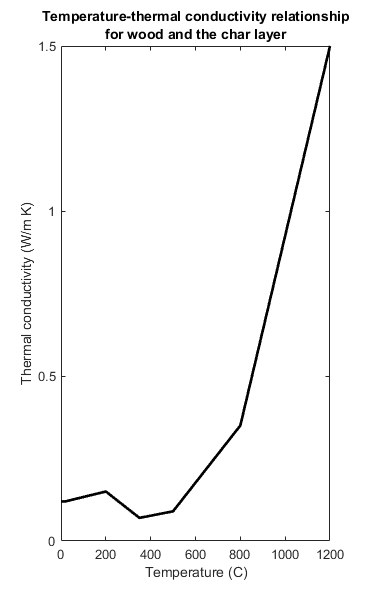
\includegraphics[width = \linewidth]{kvalues_euro.png}
	\end{figure}
	

	
\section{Program}
 \chapter{Technical Foundation} \label{tech}
%(RIJK: net 'n comment om te se ek is baie lief vir jou en baie trots op jou <3)
In this chapter, detailed explanations of the algorithms and concepts applied throughout the project are presented. 
This chapter aims to enable the reader to better understand the implementation and reasoning for the use of specific methods.
\section{Thermal properties of timber}
Specific thermal properties of timber need to be thoroughly understood to allow for accurate modelling and interpretation of the results.
After $100 ^{^\circ}$C, the temperature exposure causes the timber structure to break down in such a way that it will not return to the original state after cooling.
This breakdown is generally referred to as thermal degradation which can be broken into four categories \citep{White:2001} \citep{Shi:2021}.
These four categories are based on the different reactions that occur, and are briefly summarised below:

\begin{itemize}
\item Above 100 \textdegree C and below 200 \textdegree C, the moisture in the timber is evaporated and other non-combustible gasses are released.
\item Between 200 \textdegree C and 300 \textdegree C, carbon monoxide is released in significant quantities, and some of the timber components undergo a change in chemical composition due to the high temperatures.
\item Temperatures above  300 \textdegree C and before 450\textdegree C are significant due to the amount of flammable volatiles released and the break of carbon linkages at 370 \textdegree C.
\item At temperatures higher than 450 \textdegree C, the remaining timber is charred and any further degradation is due to oxidation from carbon monoxide, carbon dioxide, and water.
\end{itemize}
%TODO
%These phases should be clear in the results and data. (TODO add lines for phases)
As the timber clearly undergoes physical and chemical changes as temperature changes it makes sense that the thermal properties also change with temperature.
Then logically the specific heat capacity($c_p$) and density($\rho$) of timber also varies with temperature.
As the thermal conductivity and thermal diffusivity will only be assessed at specific temperatures, the specific heat and density  at only those temperatures will be summarised below.
\begin{table}[H]\label{cptab}
\centering
	\begin{tabular}{ r r r r }
	\toprule
	\multicolumn{1}{c}{Temp}& \multicolumn{1}{c}{$c_p$}& \multicolumn{1}{c}{$\rho$} & \multicolumn{1}{c}{$c_p\rho$}\\
	\multicolumn{1}{c}{\textdegree C} & \multicolumn{1}{c}{$(J/kg/K)$} &  \multicolumn{1}{c}{$(kg/m^3)$} & \multicolumn{1}{c}{$(kJ/kg/K)$}\\
	\midrule
	0   & 1530 & 479&732.8\\
	60  &1652	& 479&791.3\\
	100 &13600& 479&6514.4\\
 	140 &2090 &408&852.7\\
	200 & 2000&408&816.0\\
	350 & 850 &220&187.0\\
	500 & 1200 &142&170.4\\
	800 & 1650&110&181.5\\
	1200& 1650 &100&165.0\\
	\bottomrule
	\end{tabular}
	\caption{$c_p$ and $\rho$ at different temperatures}
\end{table}
All the thermal properties of various timber species at high temperatures were discussed in a research article by \citet{Shi:2021}.
 In their article, they provide a general expression for the thermal conductivity of softwoods (Equation \ref{softconeq}) and char (Equation \ref{charconeq}).  


 \begin{equation}\label{softconeq}
 \kappa = 0.124 +0.8432 \times 10^{-4} (\text{T}-293) 
 \end{equation}
 \begin{equation}\label{charconeq}
 \kappa = 0.091 + 8.2 \times 10^{-4} \text{T}
 \end{equation}
 
 For this project, the temperature of char will be used as 300 \textdegree C following the research of \citeauthor{Westhuyzen:2020}. 
% The specific heat ($C_p$) will be assumed to be constant at 1500 kJ/$\text{m}^3$/K. the density of pine was also assumed constant at 
 Using the equations of \citeauthor{Shi:2021}, the following $\kappa$-values (Equation \ref{shiK}) are obtained. 
\begin{equation}\label{shiK}
  \kappa=
  \begin{blockarray}{*{1}{c} l}
%    \begin{block}{*{1}{>{$\footnotesize}c<{$}} 1}
%      $\text{W/m}\cdot\text{K}$ &\\
%    \end{block}
    \begin{block}{[*{1}{c}]>{$\footnotesize}l<{$}}
     	0.0993\bigstrut[t] & 0 $^{^\circ} \text{C}$\\
		0.1044& 60  $^{^\circ} \text{C}$\\ 
		0.1077& 100 $^{^\circ} \text{C}$\\ 
		0.1111& 140 $^{^\circ} \text{C}$\\ 
		0.1162& 200 $^{^\circ} \text{C}$\\ 
		0.3780& 350 $^{^\circ} \text{C}$\\
		0.5010& 500 $^{^\circ} \text{C}$\\ 
		0.7470& 800 $^{^\circ} \text{C}$\\ 
		1.0750& 1200 $^{^\circ} \text{C}$\\
    \end{block}
  \end{blockarray}
\end{equation}
From the big difference between these values and the Euro code values, it is clear that these simple equations are not sufficient for determining the thermal conductivity of pine.
\subsection{Heat conduction and diffusion}\label{heatconsec}	 
	Heat is transferred within an element if a temperature gradient present, the rate that heat transfers is directly influenced by the thermal conductivity of the material. 
	For this project heat transferred via conduction will be focused on but heat can also be transferred in the form of thermal radiation or convection \cite{Fish:2007}.
	The heat conduction equation or Fourier's Law of heat conduction \citep{Fourier:1878} can be simply expressed in  equation \ref{fourier_eq}. 
	Where heat flux is expressed as a partial differential equation dependant on the temperature and thickness of the element. 
	More information can be added if the temperature only varies in one direction. 
	The thermal conductivity can also be expressed as a negative since heat always flows from warm to cold.
	Fourier's Law can then be written as in Equation \ref{heat_eq}
	
	
	\begin{equation}
	\label{fourier_eq}
		q = k \frac{\Delta T}{L}
	\end{equation}
	
	\begin{equation}
	\label{heat_eq}
		q = -k \frac{\partial{u}}{\partial{x}}
	\end{equation}

Derivation of the heat conduction equation over time leads to the heat diffusivity equation (Equation \ref{heatdifeq})

\begin{equation}\label{heatdifeq}
\frac{\partial u}{\partial t} = -\alpha \frac{\partial^2 u}{\partial x^2}
\end{equation}
where 
\begin{equation}\label{alphaeq}
\alpha = \frac{\kappa}{c_p\rho}
\end{equation}
From Equation \ref{alphaeq} the importance of knowing the specific heat cpacity and dentsity of the timber at different temperatures is clear.
The values in Table \ref{cptab} will be used in conjunction with the $\kappa$-values determined through simulation to calculate new thermal diffusivity values.

\section{Finite Element Method}\label{femsec}
The finite element method (or finite element analysis) is  used when the behaviour of a large element cannot be accurately depicted by a simple mathematical equation. 
Modelling the behaviour of large and complex systems is a near impossible task without breaking the problem into smaller understandable parts.
The finite element method enables engineers and scientists to break a large problem or element into comprehend-able and definable parts \citep{Zienkiewicz:2000}. 
This allows approximations and assumptions to be made at a small scale without affecting the large scale significantly, such as assuming linear behaviour between nodes. 
To understand simply why it works you could simply look at your computer screen. 
The screen consists of pixels that are simplified to one colour but the collection of pixels that is seen from the user perspective can show complex forms and pattens.
Each pixel was simplified and approximated but the end result is sufficiently accurate due to the sheer number of pixels.
Assumptions made on a smaller scale have a lesser effect on the final answer than the same assumptions made on a large scale would have had.
If the whole screen was one pixel and only the majority colour was assumed true the whole screen would be white and that is clearly incorrect. 
From that follows that the accuracy of a finite element model is very dependant on the number of elements used and only improves with more elements.
Sadly the computational time needed to analyse a model with a thousand elements is significantly more than needed for a model with less elements.
The fine balance between sufficient accuracy and short enough computational time should always be kept in mind.


	\subsection{Origin}
	The finite element method (FEM) used today is the sum of decades of research. 
	In an article by \citet{Gupta:1996}, the authors discuss the five main contributors to the finite element method. 
	They claim the idea behind the finite element method was initially explored in the \citeyear{Courant:1943} article by \citeauthor{Courant:1943}. 
	Courant acknowledges the complex nature of mathematical problems in his first paragraph by stating: "Mathematics is an indivisible organism uniting theoretical contemplation and active application."
	He goes on to discuss the variational method created by Lord Rayleigh and Walther Ritz and the shortcomings of their methods.
	He concludes that using few elements does not provide accurate local estimations but instead the interpolation will provide approximations of the actual quantities that are sufficient for engineering problems.
	As his paper did not go into depth into the calculations Courant cannot be accredited with the full development but rather with the starting point.
	In 1954 J. Argyris published an article  where the details of his calculations are clear and matrix formulation can be seen.
	The finite element method as known to day were directly defined and clarified in a text book by Zienkiewicz in 1957.
	This textbook is now in its fifth edition of print and has been continuously updated and was used for this project.
	
	\subsection{Boundaries}
	An important part of how finite element models are how the known information is embedded into the model.
	The main way this is done is by defining boundary conditions at known points. The two types of boundary conditions used in this project are Dirichlet boundaries and Newmann boundaries.
	
	Named after Johann P.G.L Dirichlet \citep{Cheng:2005}, Dirichlet boundaries force the solution function to be equal to the prescribed value at the boundary. 
	Newmann boundaries prescribe that the derivative of the solution function be equal to the predetermined value. 
	In the context of this problem, the Dirichlet boundaries prescribe the temperatures at the boundaries and the Newmann boundaries prescribe the heat flux at the boundaries.
	
%
%	\subsection{Weak form and Strong form}
%	The weak form is obtained from the balance equation and the natural boundaries\cite{Fish:2007}
%	

	
\section{Bayes' theorem of inverse problems}

%	Statistical and Computational Inverse problems by Kaipio and Somersalo Chapter 3
% 	The Bayesian approach to Inverse Problems Dashti and Stuart
	The method of statistical inversion is dependant on a fundamental understanding of the Bayes' theorem of inverse problems. 
	The student obtained this understanding through studying Chapter 3 of statistical and Computational Inverse problems by \citet{Kaipo:2005}, further referred to merely as Kaipio. 
	There are four principles of Statistical inversion that is essential to the thorough understanding of these models. 
	Firstly, it is the principle that any variable in the model needs to be modelled as a random variable. 
	This randomness is based on the extent of information that is available. 
	To ensure that the extent of knowledge is accurately portrayed in the model, the extent of knowledge will be coded into the probability distributions assigned to the different variables. 
	Finally, it needs to be understood that the solution of a statistical inversion is a posterior probability distribution.
	A generalized equation of Bayes' theorem can be seen in \ref{bayes_eq} taken from Kaipio. 
	
	\begin{equation}
	\label{bayes_eq}
	\pi_{\text{post}}(x) = \pi(x|y_{\text{observed}}) = \frac{\pi_{\text{pr}}(x) \pi(y_{\text{observed}}|x)}{\pi (y_{\text{observed}})}	
	\end{equation}
	
Further application of Bayes' theorem of inverse problems to the project at hand is discussed in Section \ref{secInvmet}
\section{Markov Chain Monte Carlo} \label{MCMCdet}
Markov Chain Monte Carlo (MCMC) is a method of integration that will be used to determine the mean of the $\kappa$-values at specific temperatures. 
	Markov Chain Monte Carlo is a method that was created by combining the concept of Monte Carlo sampling  and a Markov Chain. 
	To fully understand MCMC, its underlying methods must be investigated further.
	For a better understanding of this concept, \textit{Introducing Markov chain Monte Carlo} by \citeauthor{Gilks:1996}, Kaipio, and various websites \citep{MLM:2019}, \citep{dummies:2015} were consulted.(RIJK: is sin lomp?)
	\subsection{Markov Chains}	\label{markovexpl}
	The core principle of a Markov chain is that the next value ($x_{n+1}$) in a sequence is dependent on the current value($x_n$). 
	A step size that indicates the range within the next point falls in.
	Values are then randomly generated but restricted to be within this range.
	This concept can be visualised as follows: the accepted point ($x_1$) is in the centre of a cube. The next possible random point is randomly generated but still within the cube(our search range). 	
	After this next number is selected, the cube moves such that the new point($x_2$) is now the centre, and so it continues.
	See Figure \ref{cubeexplfig} for clarification.
	The above example simplifies the concept, but this understanding can now be expanded.
	If every coordinate direction in the aforementioned simple example is seen as a single entry in the $x$ vector, then the example has three independent values.
	More or fewer values can be used depending on the problem.
	Another level of complication can be added if it is taken into account that every point in the cube is no longer equally likely.
	A distribution within the cube can be chosen, for example simply a normal distribution
	The shape of the cube then warps into a stranger shape with points closer to the center being more likely choices and the edges being less likely.
	\begin{figure}	
	\centering
	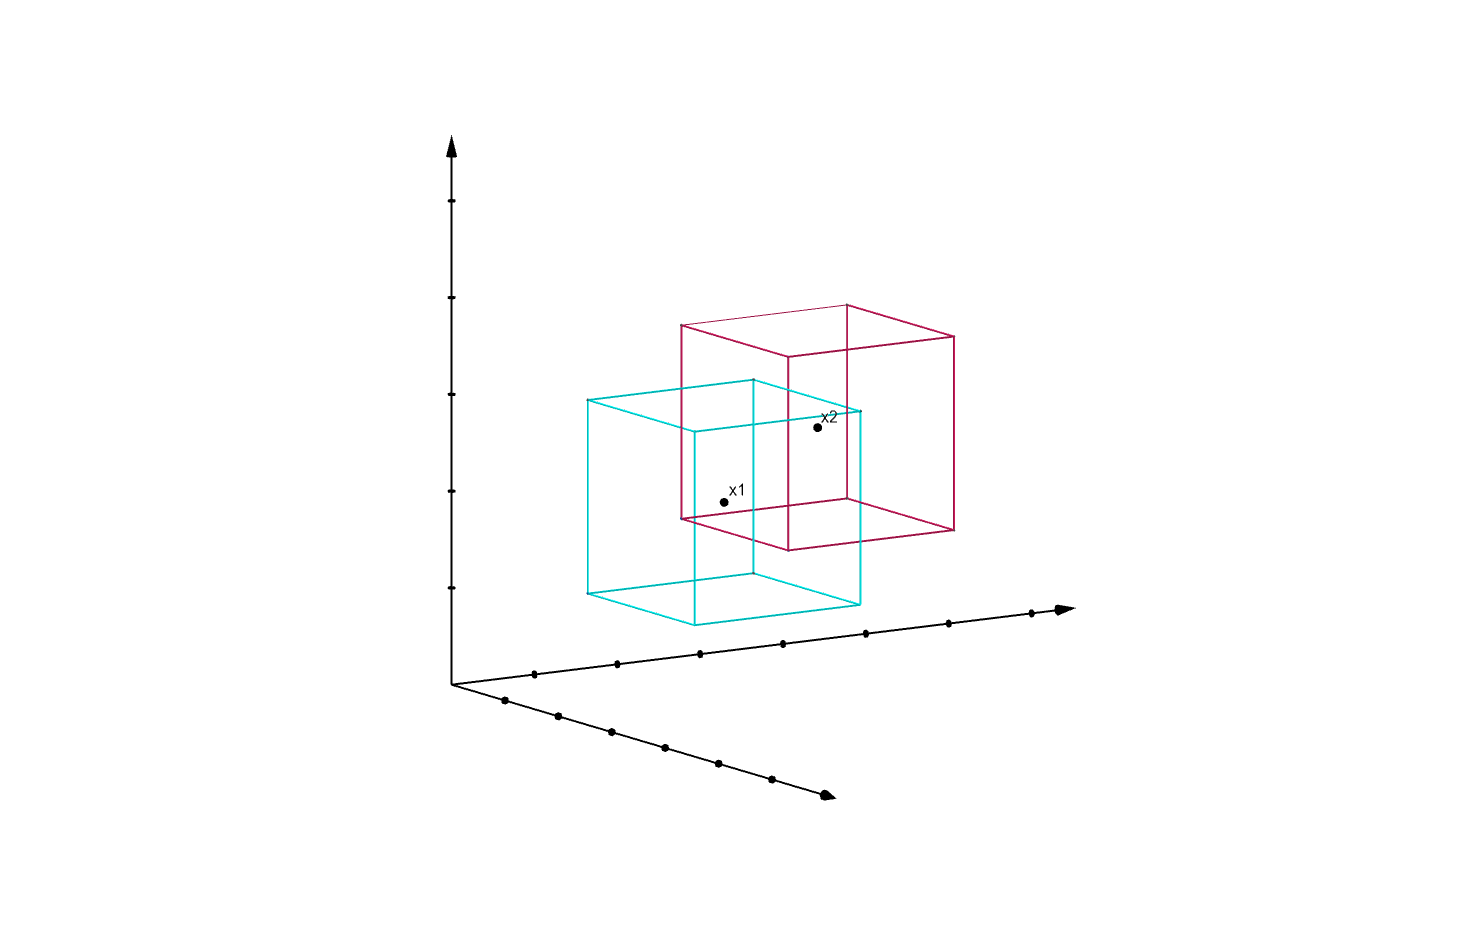
\includegraphics[width=0.55\linewidth]{figures/MC_cubes.png}
	\caption{Three-dimensional example of Markov Chain application (Created on \url{https://www.geogebra.org/3d})}
	\label{cubeexplfig}
	\end{figure}
	
	%%BURN_IN TODO
	The purpose of a Markov Chain is for the chain to converge to a distribution and be independent on the very initial estimation. 
	In principle, it should then reach a near stationary distribution.
	Since Markov Chains are not used if we know the answer, a way to determine when values are no longer affected by the initial estimate is needed \cite{Gilks:1996}. 
	The simple proposed solution is the concept of burn-in. 
	The concept of conventional burn-in for usage in Markov Chains are disputed as the Markov Chain itself is created in such a way that values are only directly dependent on the value immediately before them \cite{Meyn:1993}.
	Burn-in in the Markov Chain sense can simply be referred to as the removal of the initial samples of low probability to increase the accuracy of the average taken after all the iterations \cite{John:2016}.
		
	\subsection{Monte Carlo Integration}\label{MCint_sec}
	Monte Carlo integration is used to evaluate a probability distribution that cannot be solved simply. 
	The evaluation is done by drawing a collection of random values from the distribution.
	These values are then used as the sample, and a sample mean is taken.
	The arithmetic sample mean can be used to approximate the population mean per the law of large numbers \citep{Gilks:1996}.
	

\subsection{Metropolis-Hastings Algorithm}

The Metropolis-Hastings algorithm is one of the available simulation methods based on the MCMC principles. 
For this project, the Metropolis-Hastings algorithm was chosen above the Gibbs-sampler as the Gibbs sampler can be relatively slow \cite{Murphy:2012}.

All of the random samples generated by the Monte Carlo integration can not be immediately accepted.
	Here, the acceptance criterion comes into play.
	There are multiple options for how a posterior is deemed acceptable; these are elaborated on in the book  \textit{Monte Carlo Statistical Methods} by \citeauthor{Robert:2004}. 
	The most general acceptance criterion is set out in Equation \ref{acceptcriteq} and comes from Kaipio.
	
		\begin{equation} \label{acceptcriteq}
		\begin{aligned}
		&\text{if  }\quad \frac{\pi (x_2)}{\pi(x_1)} > 1 \quad \text{Accept automatically}\\
		&\text{or  }\quad \frac{\pi (x_2)}{\pi(x_1)} > \text{rand}  \quad \text{Accept}\\
		&\text{else reject and reselect  } x_2
		\end{aligned}
		\end{equation}

\section{Maximum a Posteriori}
To ensure a thorough investigation of the thermal diffusivity of timber the posteriori function will also be optimised to obtain the value with the highest probability, maximum a posteriori, in addition to the mean.
As the implementation will be done using built-in optimisation functions in Matlab the technical aspects will briefly explain how that function works.
The function used is \texttt{fminsearch.m}.
In the name of the function, it can be seen that the function will be minimised.
This seems counter-intuitive since the intention is to find the maximum of the function. 
Luckily the minimum is simply a negative maximum. 

According to the \texttt{fminsearch} Matlab documentation (\url{https://ch.mathworks.com/help/matlab/ref/fminsearch.html}) , the algorithm is based on the Nelder-Mead algorithm \citep{Lagarias:1998}.
The Nelder-Mead algorithm is an unconstrained heuristic direct search method.
The heuristic aspect of the algorithm means that it searches the function space in a guided random manner.

Nelder-Mead uses a simplex, a triangle in the dimension needed, to find the minimum.
In two-dimension, the simplex is simply a triangle, where each point has a $x$ and $y$ coordinate and is notated as. 
A starting value needs to be provided to the algorithm, this will then be one of the points in the first simplex.
All the points on the simplex are ordered from best to worst, where the smallest value ($f(x)$) is best if minimising.
In the two-dimensional example, the centroid of the two best points ($x_l,x_s$) are calculated, from there using the value of the function at the simplexes and the centroid transformations can be performed to find even smaller values.
The transformations are applied to change the worst point ($x_h$) until it is no longer the worst.

The transformations are performed in a specific order.
The first transformation is reflection.
Point $x_h$ is mirrored around the line that passes through the centroid and $x_l$ and $x_s$ to create $x_r$.
The idea behind this is that the values are lower in that direction so the algorithm attempts to take the biggest stride possible to a lower value.
If $x_r$ is better than $x_r$  the triangle is expanded and $x_e$ is even further in the assumed minimising direction.
If $x_r$ is not better than $x_h$, the reflected point is rejected and the original $x_3$ is contracted closer to $x_1$ and $x_2$.
This contracted point ($x_c$) should ideally have a smaller value than $x_h$, if not a shrink contraction needs to be performed.
In a shrink contraction, $x_h$ and $x_s$ are redefined and pulled closer to $x_l$ with hopes of finding the minimum near the best point.

The result is a simplex that moves over a surface in search of the lowest point and as it reaches that point it shrinks until all the points are practically at the same place. When this happens or the points are close enough to each other as defined when initializing the code the algorithm stops. Below in Figure \ref{neldermeadfig}, the different transformations can be seen.

\begin{figure}\label{neldermeadfig}
\centering
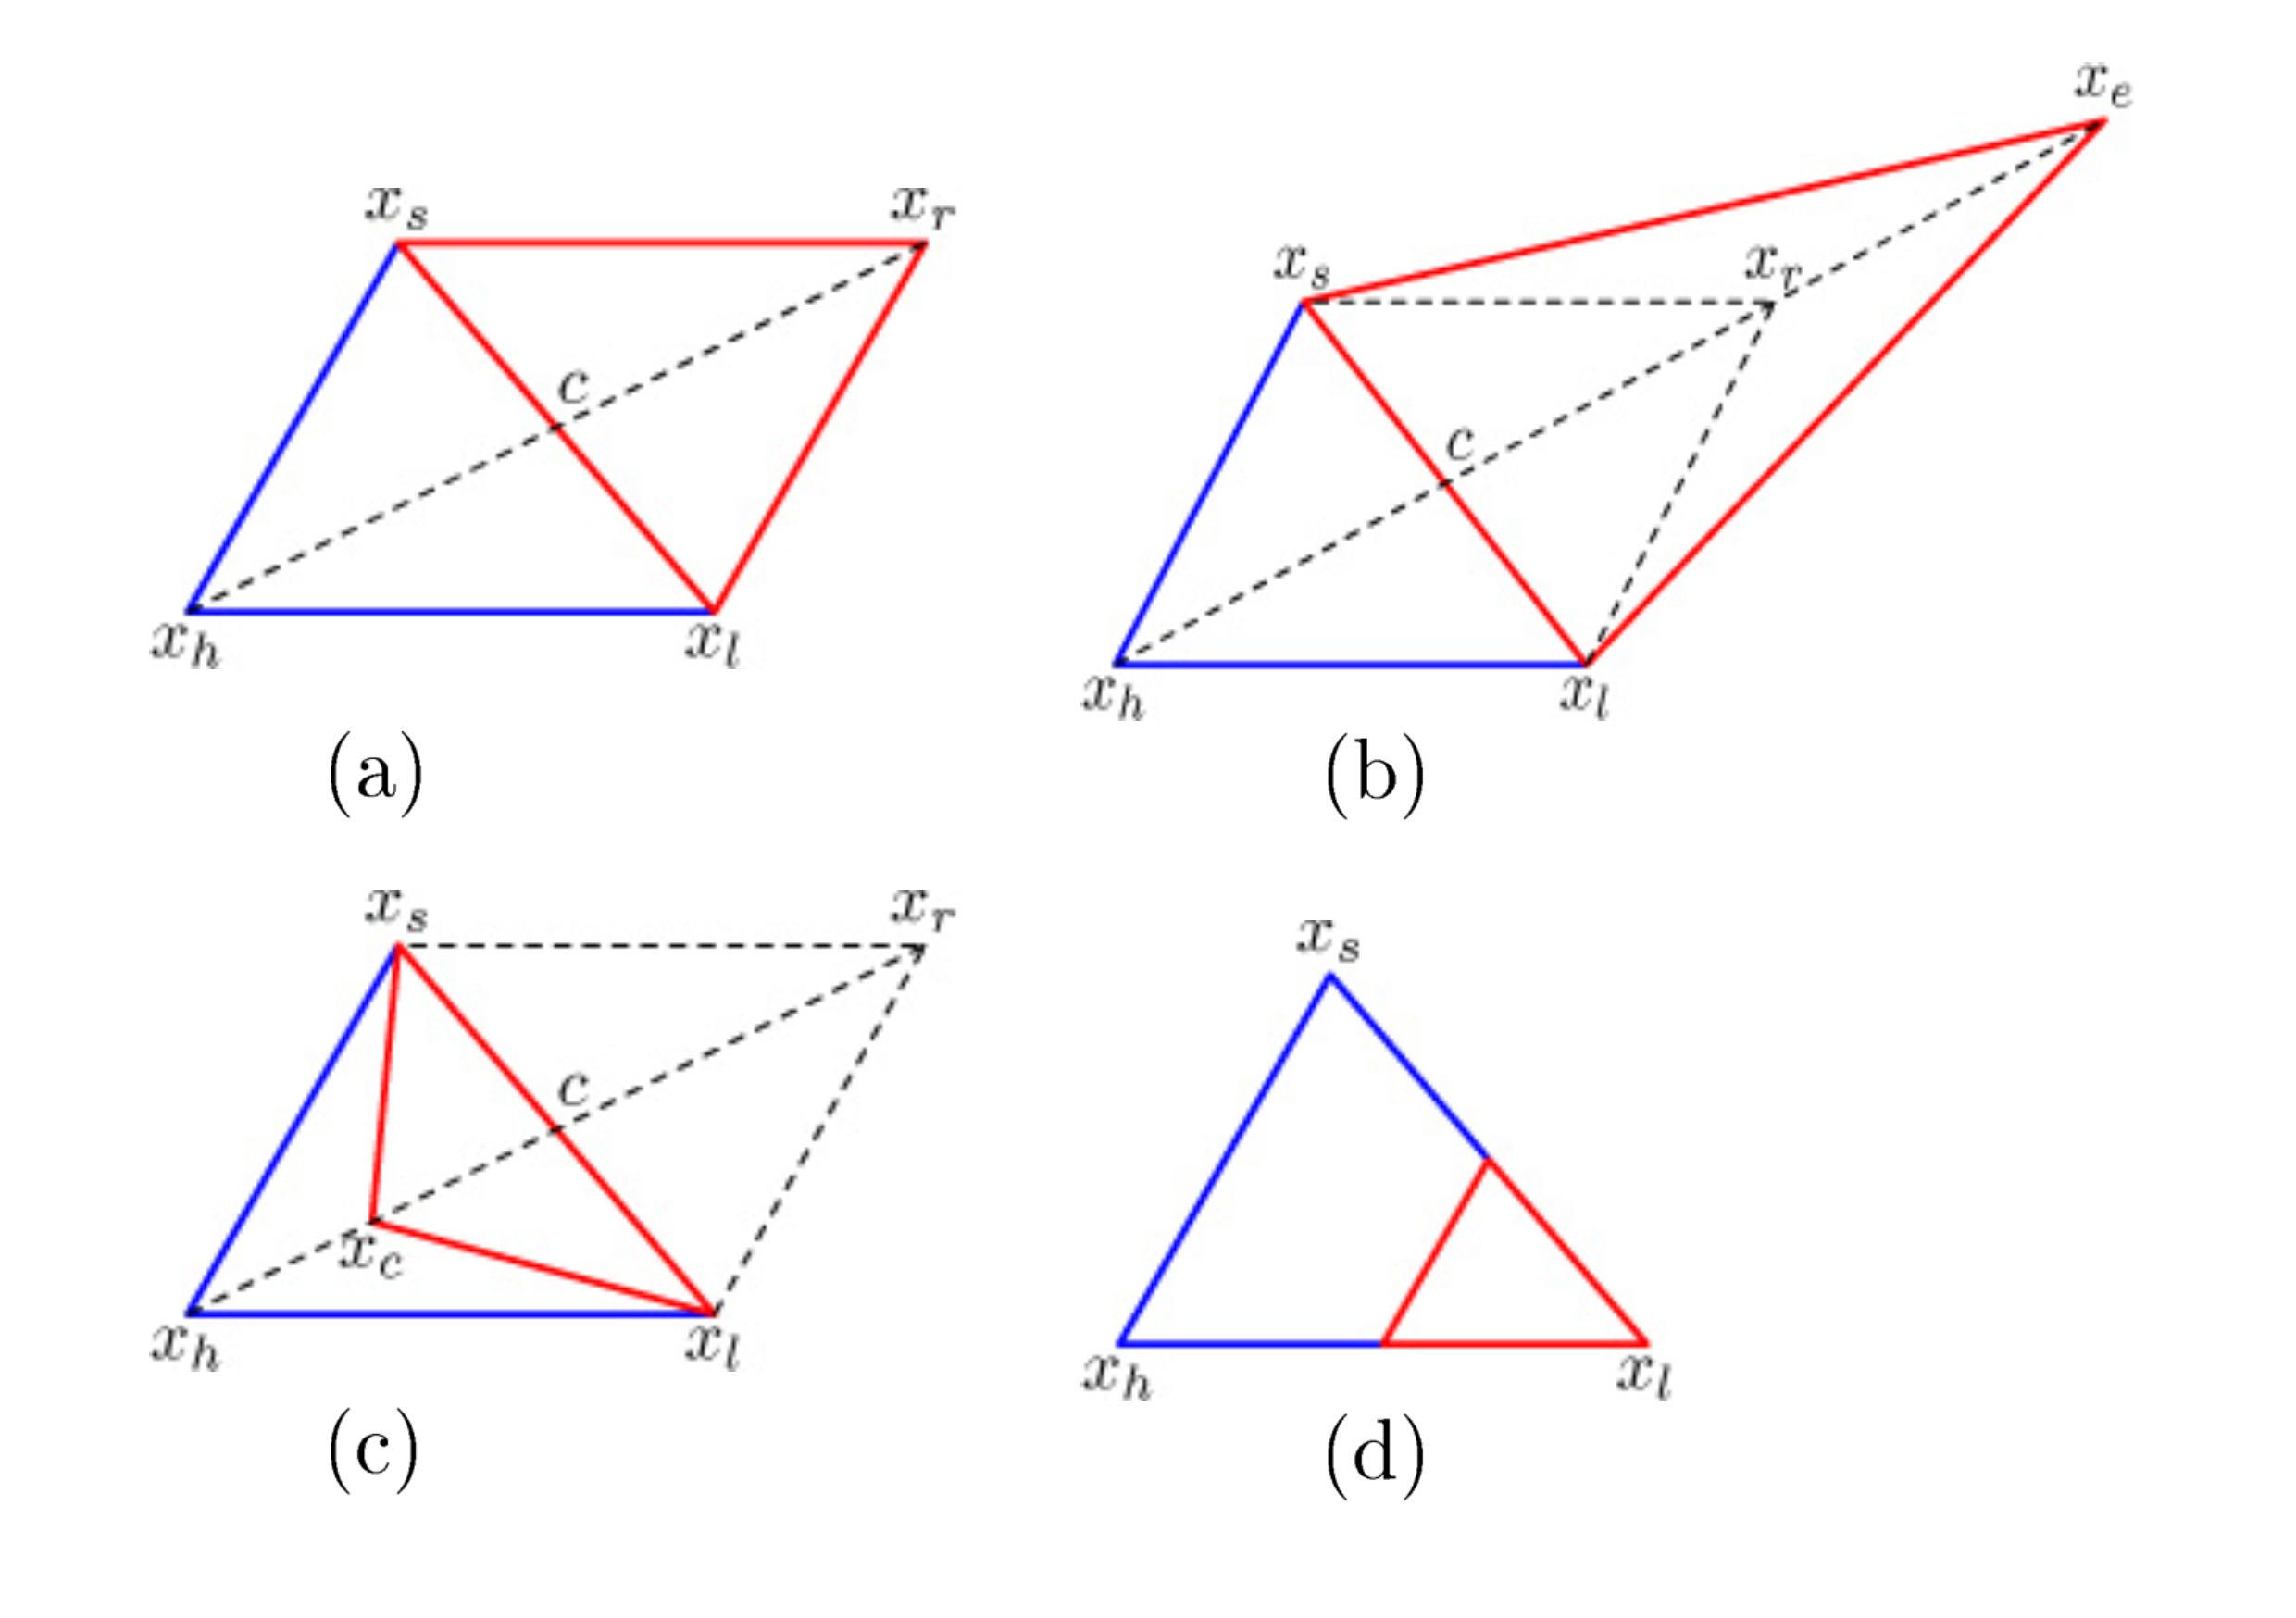
\includegraphics[width=\linewidth]{figures/MAP_expl.png}
\caption{Visual representation of Nedler-Mead transformations a) Reflection, b) Expansion, c) Contraction, d) Shrink contraction (Source:\url{https://codesachin.wordpress.com/2016/01/16/nelder-mead-optimization/})}
\end{figure}

%gramarly done 17/10


 \chapter{Implementation}
\section{Measured Data}
	\subsection{Summary of test}
	The data used was acquired by \cite{Westhuyzen:2020} for an article assessing the charring rate of both SA-Pine and Eucalyptus.
	For the purpose of this project only the data obtained from the SA-Pine test was considered and analysed. 
	The test sample was a 100 mm by 0.9m x 0.9m panel of cross-laminated SA-pine, this sample was then divided into nine cubes of 100 mm x 100 mm x 100 mm.
	Each cube was fitted with seven Type K-thermocouples placed at consecutive 16.5 mm drilled holes.
	The test panel was tested in a furnace and was exposed to the standard ISO 834 Fire curve \ref{firecurve_fig} on one side and room temperature on the other. 
	The panel was exposed to the fire curve for 50 minutes at which stage near complete de-lamination was observed and the test ended.
	
	
	\begin{figure}[H]
	\centering 
	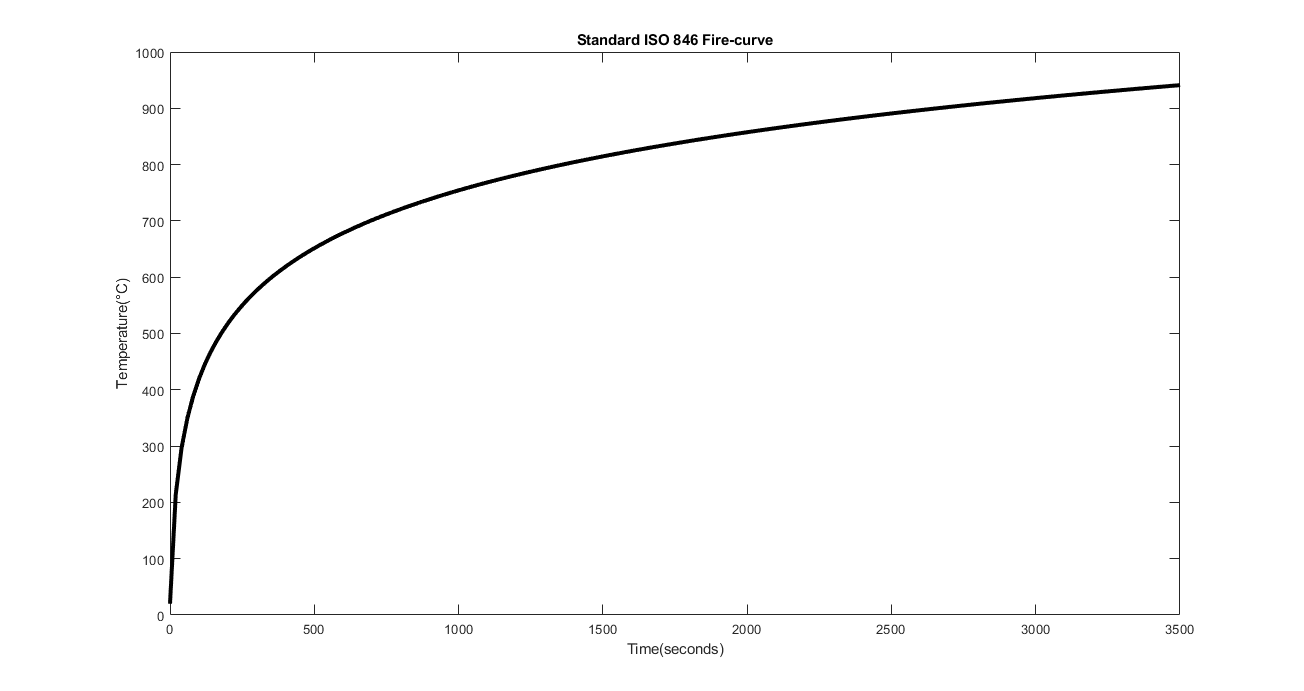
\includegraphics[width=\linewidth]{firecurve.png}
	\caption{Standard ISO fire curve TODO}
	\label{firecurve_fig}
	\end{figure}
	
	\subsection{Potential inaccuracies}
	As with most test everything is not always perfect. 
	In the data it was observed that two of the thermocouples broke during testing, this resulted in temperature with a magnitude of $10^{13}$. 
	That temperature is not possible as the highest ever recorded temperature reached was $4\text{x}10^{12}$ and that only occurred in a atomic explosion %(https://www.insidescience.org/news/hottest-temperature-universe-measured)% 
	This malfunction required that two of the depth measurements were no longer the average between nine samples but instead the average between eight.
	
	Another inaccuracy that could potentially influence the accuracy of the final result is the accuracy of the depth of the holes in which the thermocouples were placed. 
	As this was done by hand. %in the laboratory.
	
	There is also debate about the significance of the contribution of the timber burning to the temperature inside the furnace. 
	For the purposes of this project it will be assumed that the timber burning does not contribute to the temperature inside the furnace.
	
	The assumption that the panel is constantly at room temperature on the outside is also inaccurate as there is heat radiating from the panel that increases the temperature surrounding the panel.

\subsubsection{Results}

\begin{figure}[H]
	\label{measured_fig}
	\centering
	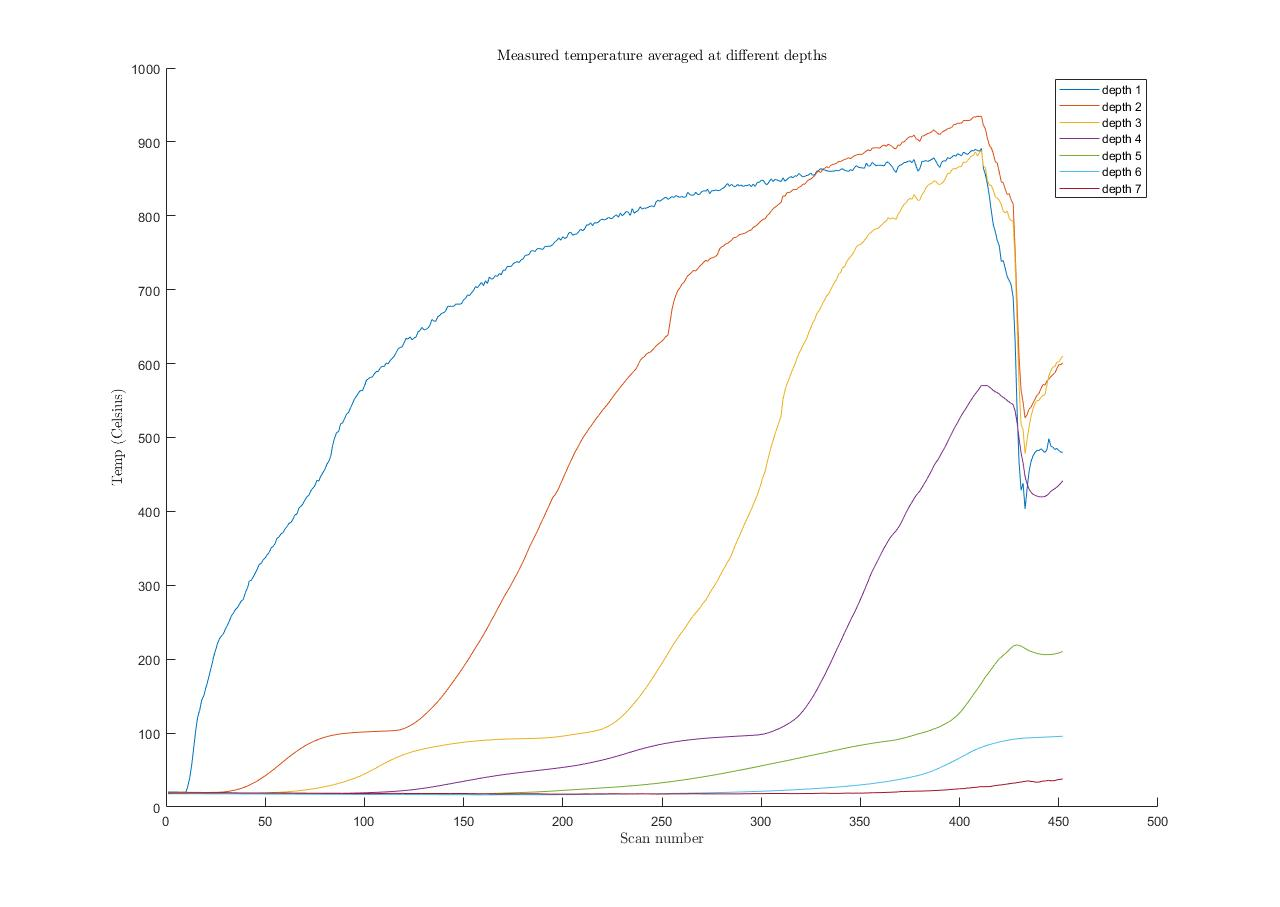
\includegraphics[width=5.5in,]{measured_data.jpg}
\end{figure}


\section{Inversion method}
%here we will discuss everything that we did
 \chapter{Results} \label{results}
The results of the MCMC analysis as well as the MAP optimization is visualised in the section below.
\section{Continuous output}
To assess the progress of the MCMC analysis while iterating, graphs similar to those in Figure \ref{fig:10} were continuously generated. 
In Figure \ref{fig:10} the output of 2000 iterations were extracted to allow sufficient detail to be visible.
Figure \ref{fig:10a} was important to keep track of the number of different samples assessed until an acceptable sample was found.
If a large number of samples were consistently needed, it could indicate that a bad starting point was chosen or that there is an error within the posterior distribution calculation.
The connection between Figures \ref{fig:10b} and \ref{fig:10c} can be seen in that when there is a dip in the difference between $\pi^*(x)$ and $\pi^*(x_{\text{ref}})$ there is a peak in the acceptance ratio.
When the graph in Figure \ref{fig:10b} is at 0 that means that the sampled values are the same as the Eurocode reference values.
When this graph is below 0 that indicates that the values sampled for that iteration produced a less likely result than the reference values.
This influenced the burn-in period chosen, to ensure that all the samples considered were more accurate than the Eurocode values.
As the probability function used is not normalised it can produce posterior probabilities larger than 1 therefore the difference between two posterior can also be larger than 1.
This also means that the higher the difference between $\pi^*(x)$ and $\pi^*(x_{\text{ref}})$ the more accurate the $x$ value is.

\begin{figure}
	\centering
	
	\begin{subfigure}[b]{\textwidth}
	\centering	
	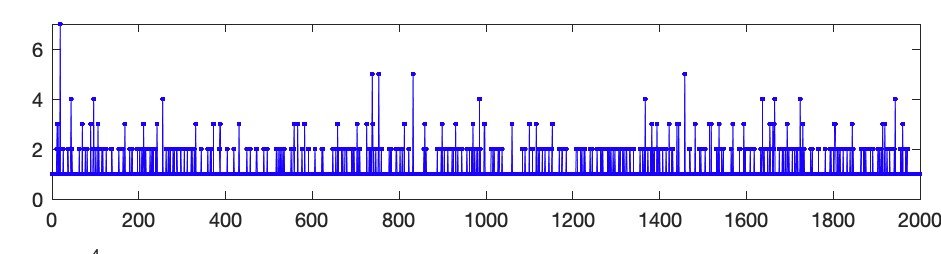
\includegraphics[width = \textwidth]{figures/figure10a.jpg}
	\caption{Number of samples drawn before an acceptable sample was found per iteration}
	\label{fig:10a}
	\end{subfigure}{}
	
	\begin{subfigure}[b]{\textwidth}
	\centering	
	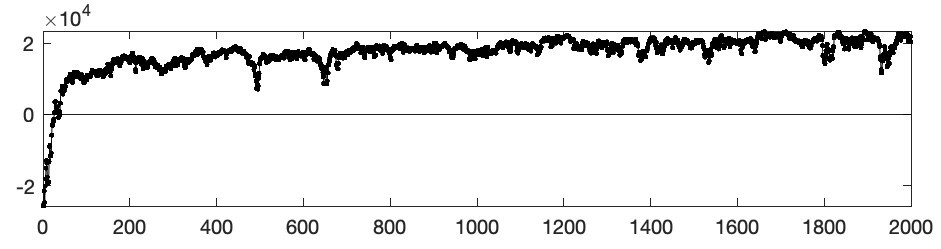
\includegraphics[width = \textwidth]{figures/figure10b.jpg}
	\caption{Difference between the accepted $x$ posterior and the reference posterior for each iteration}
	\label{fig:10b}
	\end{subfigure}{}
	
	\begin{subfigure}[b]{\textwidth}
	\centering	
	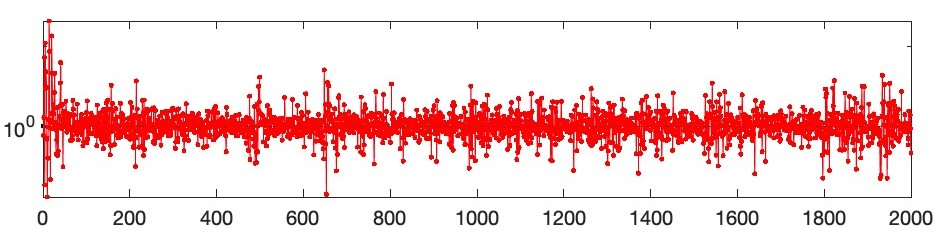
\includegraphics[width = \textwidth]{figures/figure10c.jpg}
	\caption{Value of acceptance ratio at each iteration}
	\label{fig:10c}
	\end{subfigure}{}
	
	\caption{Graphs from continuous output}
	\label{fig:10}
\end{figure}



\section{Resulting \texorpdfstring{$\kappa$}{TEXT}-values}

The thermal conductivity ($\kappa$-values) at key temperatures integral to this project, the resulting values are shown in Table \ref{krestab}. 
As can be seen in Figure \ref{kresult_euro_fig} there was quite a drastic difference in the thermal diffusivity at 1200 \textdegree C and between 0\textdegree C and 200\textdegree C.
The large difference at 1200\textdegree C is due to how the model is created, at that temperature the majority of the heat is transferred through thermal radiation.
The model did not model thermal radiation separately but instead incorporated the radiation into a equivalent conduction.
Between 0\textdegree C and 200\textdegree C the modelling of the evaporation was moderately successful as a spike can be seen at 100 \textdegree C.  
\begin{figure}
\centering	
	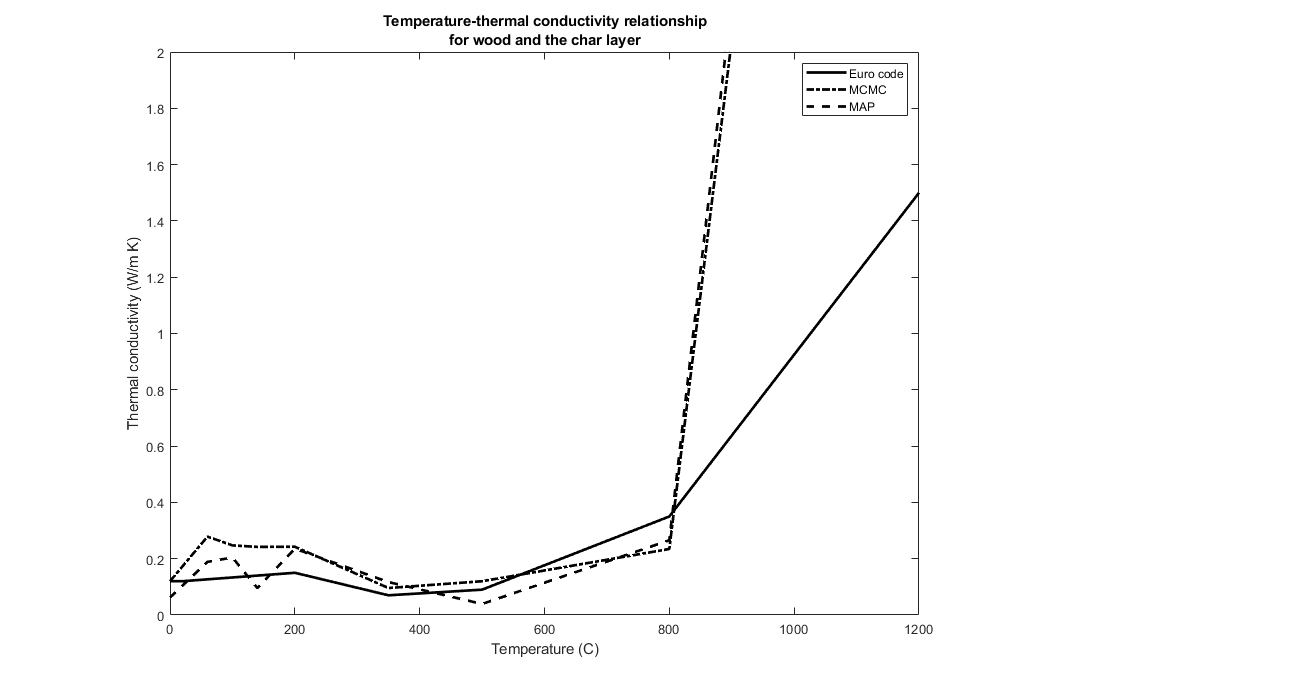
\includegraphics[width=\textwidth]{figures/kvalues_all_NOshi.png}
	\caption{Resulting $\kappa$ values compared to Eurocode standard values}
	\label{kresult_euro_fig}
\end{figure}
\begin{table} 
\centering
\caption{Posterior thermal conductivity in W/(m$\cdot$K)}
\label{krestab}
	\begin{tabular}{ r r r r }
	\toprule
	 \textdegree C & EURO & MAP & MCMC\\
	\midrule
	0   & 0.12&0.062 &0.12\\
	60  &0.12& 0.189 &0.278\\
	100 &0.12& 0.204 &0.247\\
 	140 &0.12& 0.096 &0.242\\
	200 & 0.15& 0.236 &0.243\\
	350 & 0.07& 0.117  &0.096\\
	500 & 0.09& 0.039 &0.120\\
	800 & 0.35& 0.265 &0.234\\
	1200& 1.5& 7.943 &7.467\\
	\bottomrule	
	\end{tabular}
	
\end{table}
 
 For each temperature there will be a different distribution of samples. 
 In Figure \ref{fig:scatdata} The distribution of all the samples were plotted in a scatter plot.
 The resulting $\kappa$-values from the MCMC algorithm is plotted in red and the Maximum a posteriori is plotted in blue.
 The non-symmetrical distribution  is clear in the data as the Maximum a posteriori is not in the centre of each distribution.

%TODO
From the difference between the histogram maximum and the maximum found by the Nelder-Mead optimization at 140\textdegree C (Figure \ref{fig:histo}) it is clear that many more iterations of the MCMC algorithm is needed.
In contrast at 60\textdegree C the maximum of the histogram and the MAP is the the same indicating that the samples at that specific temperature was sufficiently explored.
An estimated 100 000 iterations would be needed.
As the current iterations already took four days an additional sixteen days would have been needed to generate the needed additional samples.
This would have been impractical to achieve during a single semester as these iterations needed the full computational capacity of the available laptop and prevented any other usage of the laptop.

\begin{figure}

\centering
	\begin{subfigure}[b]{0.45\linewidth}
	\centering
	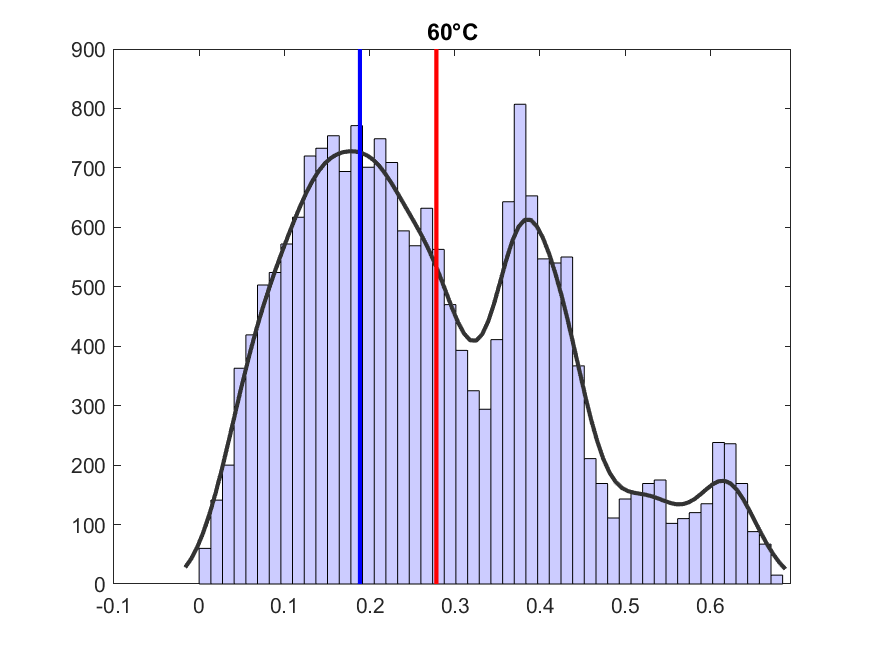
\includegraphics[width = \linewidth]{figures/histograph/histo1.png}
	\end{subfigure}
	\begin{subfigure}[b]{0.45\linewidth}
	\centering
	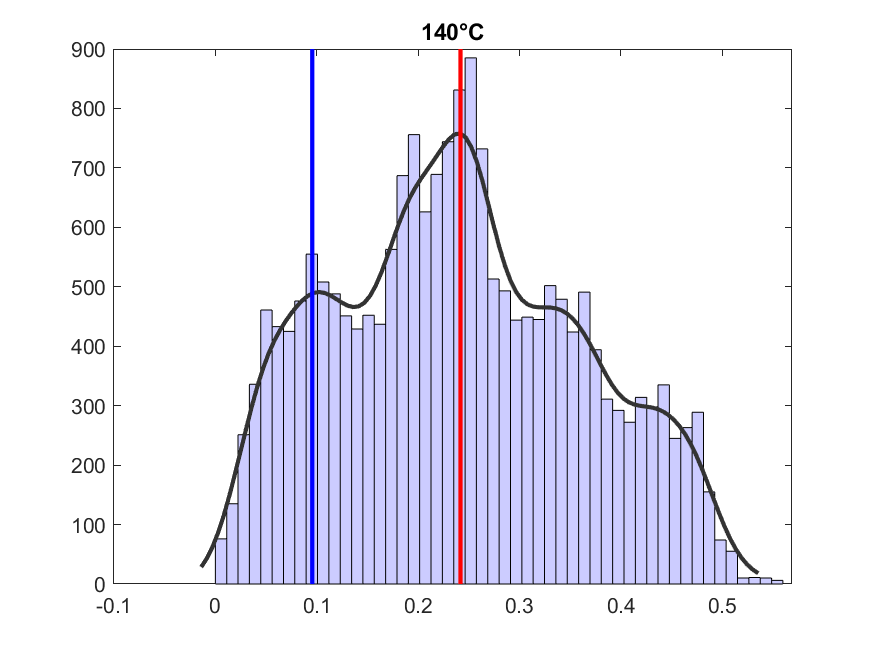
\includegraphics[width = \linewidth]{figures/histograph/histo3.png}
	\end{subfigure}
	\centering
	\begin{subfigure}[b]{0.2\linewidth}
	\centering
	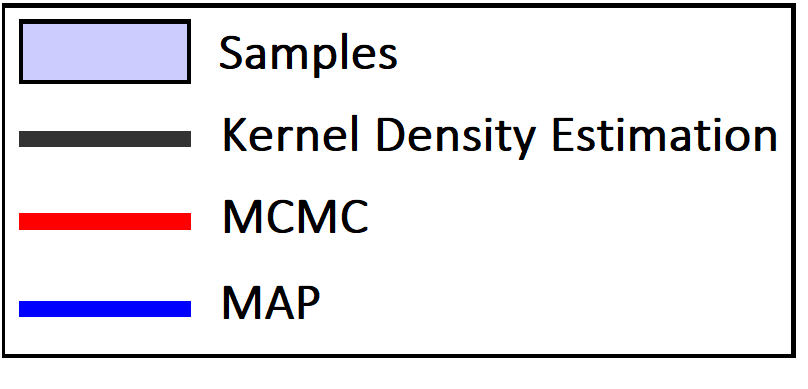
\includegraphics[width = \linewidth]{figures/histograph/legend.png}
	\end{subfigure}
	\caption{Distribution of samples at 60\textdegree C and 140\textdegree C with MCMC and MAP results indicated}
	\label{fig:histo}
\end{figure}

%\begin{figure}[b]
\label{histofig}
\centering
	\begin{subfigure}{}
	\centering
	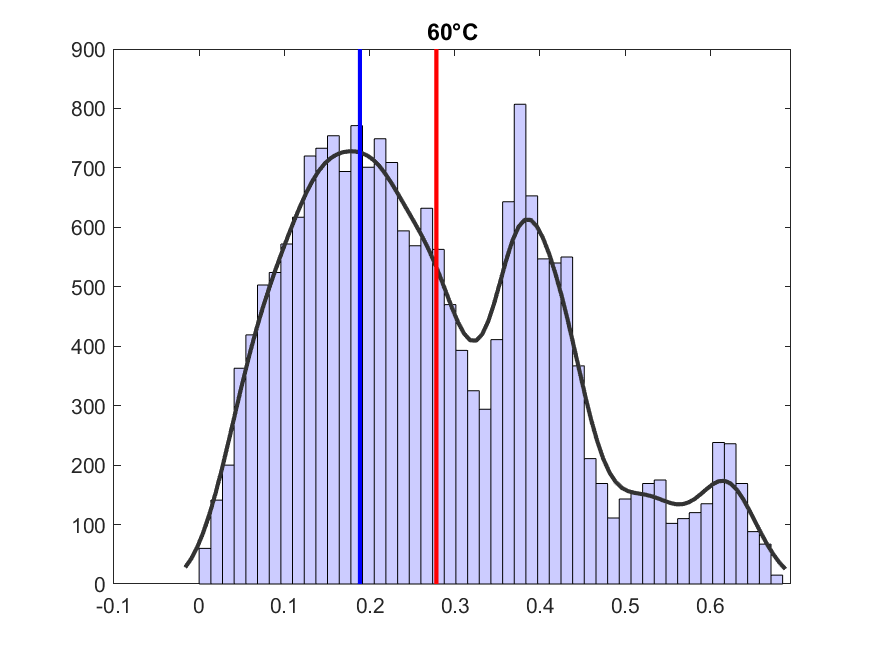
\includegraphics[width = 0.45\linewidth]{figures/histograph/histo1.png}
	\end{subfigure}
	\begin{subfigure}{}
	\centering
	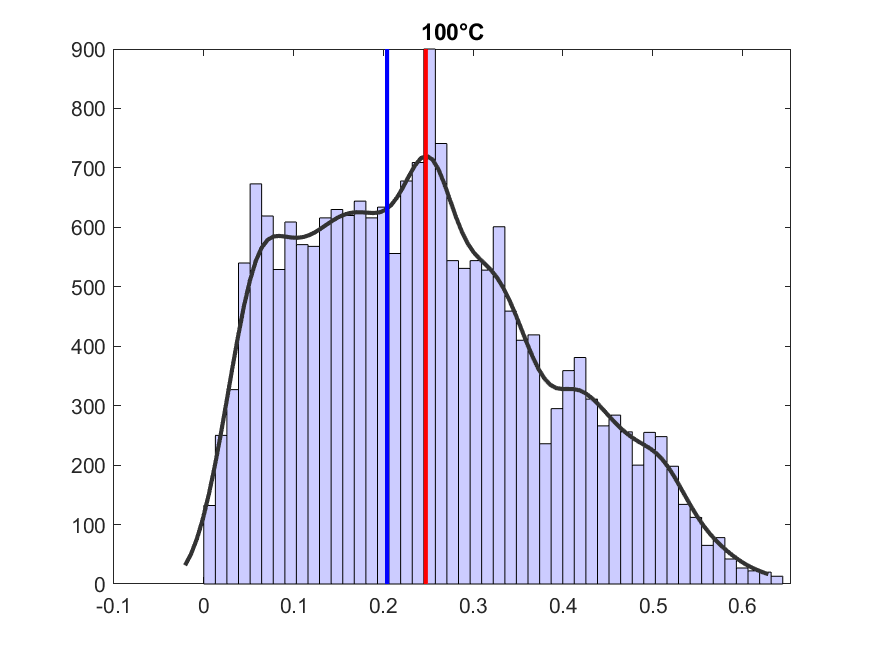
\includegraphics[width = 0.45\linewidth]{figures/histograph/histo2.png}
	\end{subfigure}
	\begin{subfigure}{}
	\centering
	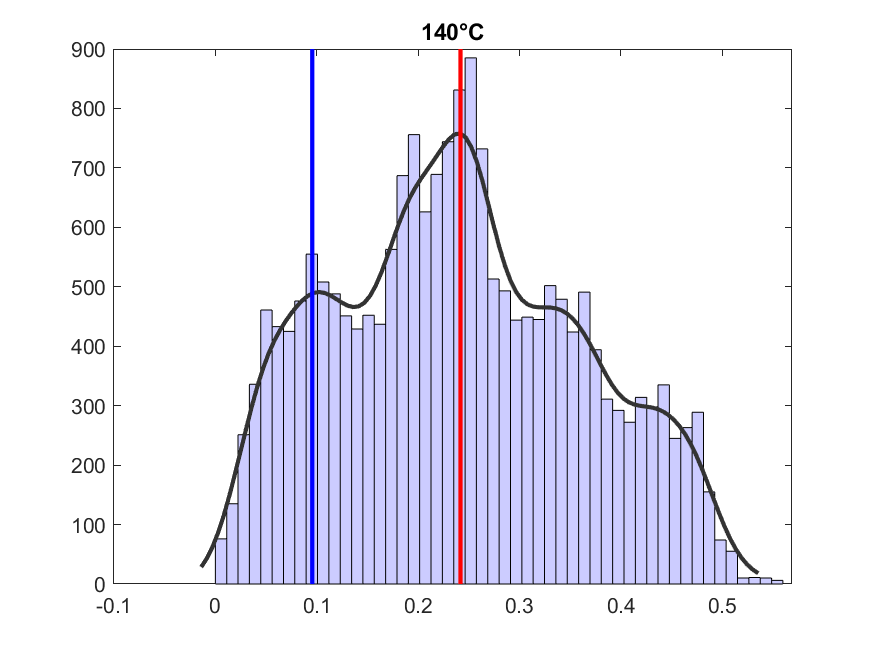
\includegraphics[width = 0.45\linewidth]{figures/histograph/histo3.png}
	\end{subfigure}
	\begin{subfigure}{}
	\centering
	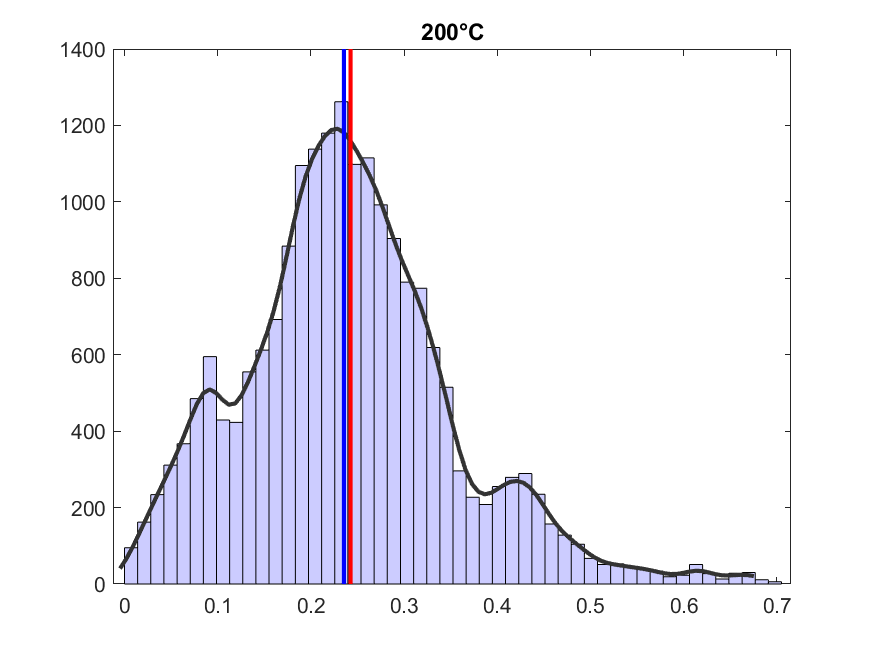
\includegraphics[width = 0.45\linewidth]{figures/histograph/histo4.png}
	\end{subfigure}
	\begin{subfigure}{}
	\centering
	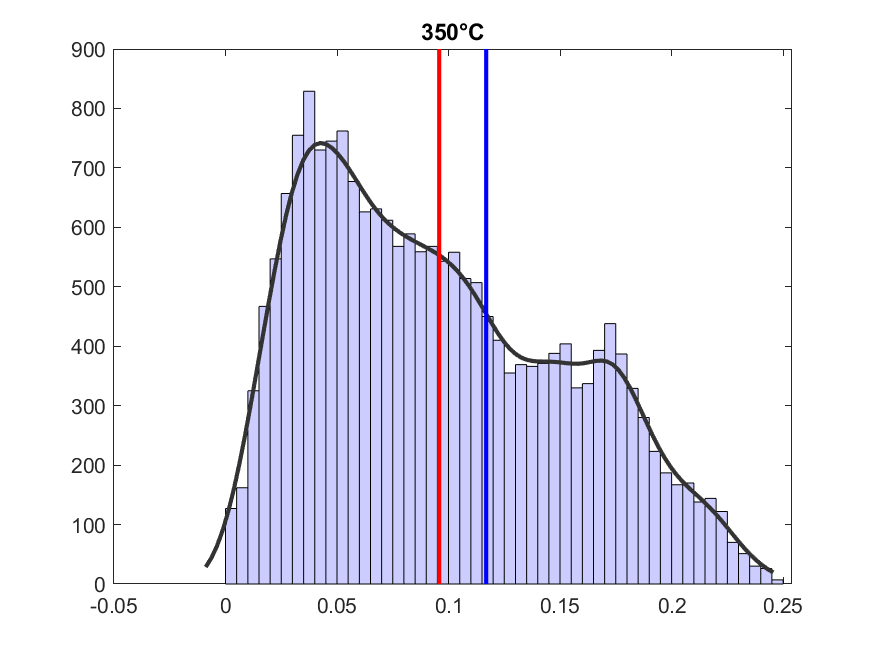
\includegraphics[width = 0.45\linewidth]{figures/histograph/histo5.png}
	\end{subfigure}
	\begin{subfigure}{}
	\centering
	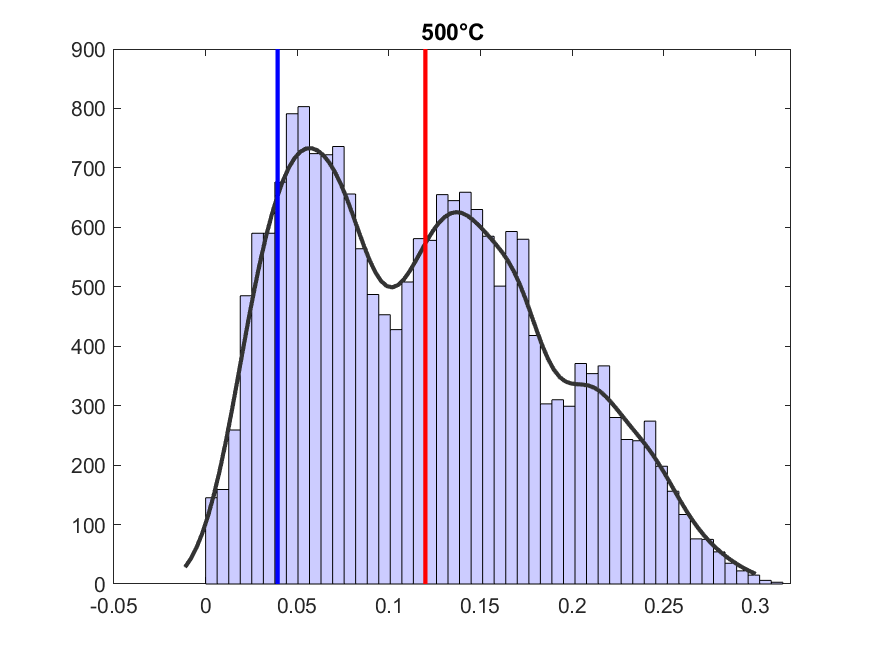
\includegraphics[width = 0.45\linewidth]{figures/histograph/histo6.png}
	\end{subfigure}
	\begin{subfigure}{}
	\centering
	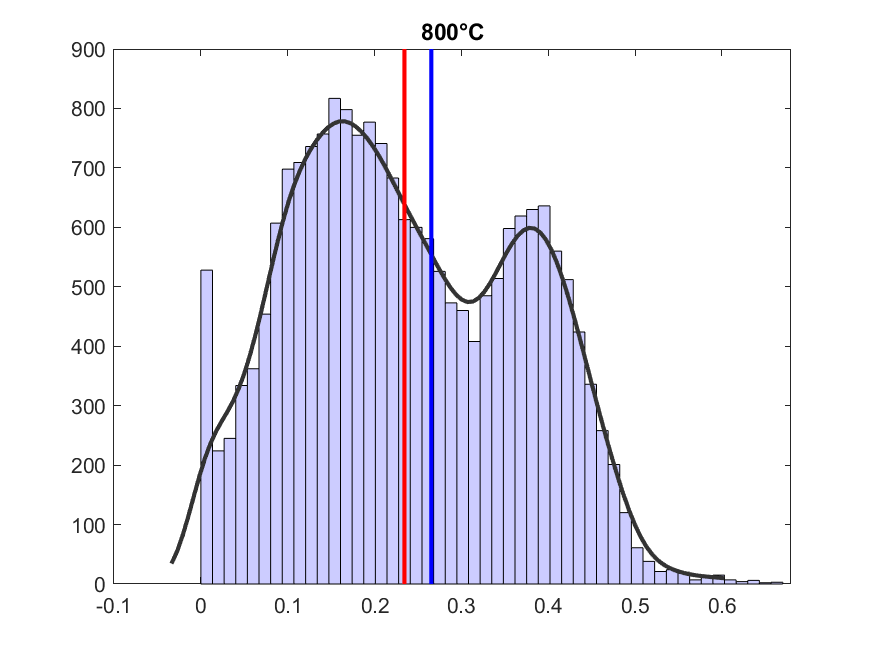
\includegraphics[width = 0.45\linewidth]{figures/histograph/histo7.png}
	\end{subfigure}
	\begin{subfigure}{}
	\centering
	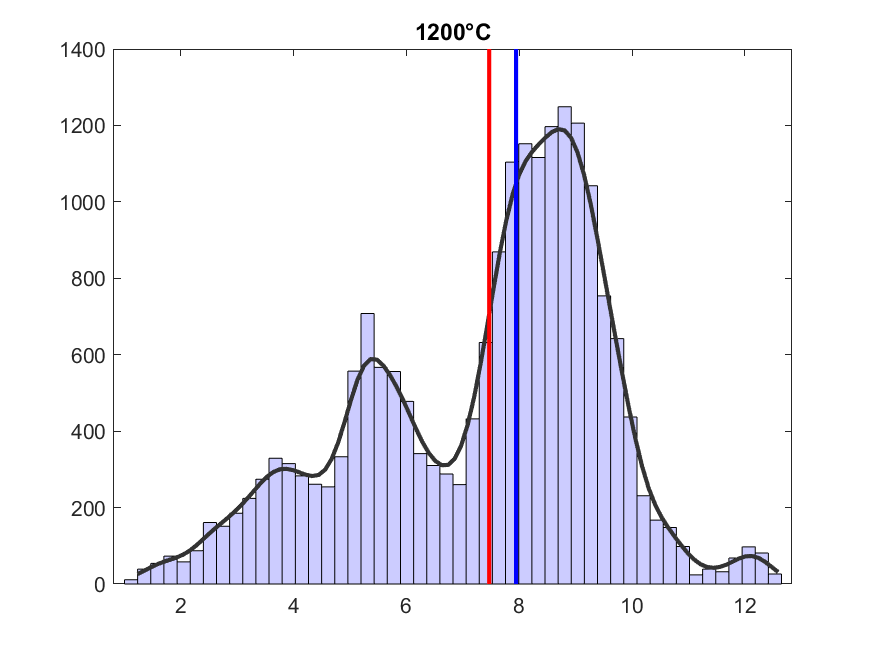
\includegraphics[width = 0.45\linewidth]{figures/histograph/histo8.png}
	\end{subfigure}
	\centering
	\begin{subfigure}{}
	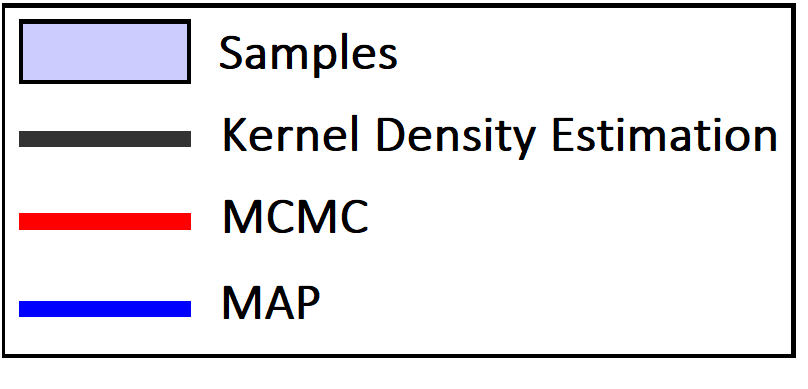
\includegraphics[width = 0.3\linewidth]{figures/histograph/legend.png}
	\end{subfigure}
	\caption[short]{Distribution of samples at different temperatures with MCMC and MAP results indicated}
\end{figure}
\begin{figure}[b]
\label{fig:scatdata}
\centering
	\begin{subfigure}{}
	\centering
	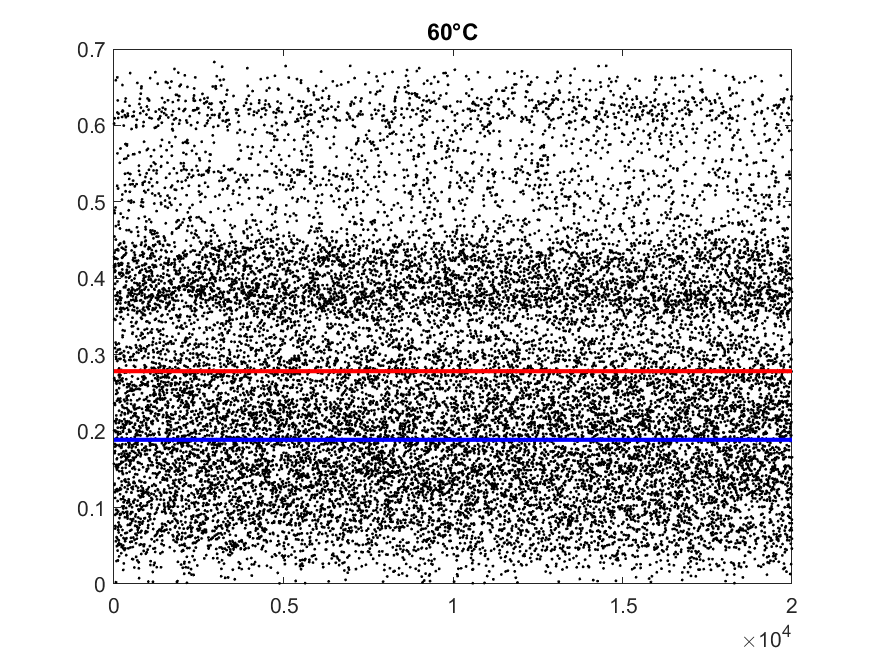
\includegraphics[width = 0.45\linewidth]{figures/histograph/scatter1.png}
	\end{subfigure}
	\begin{subfigure}{}
	\centering
	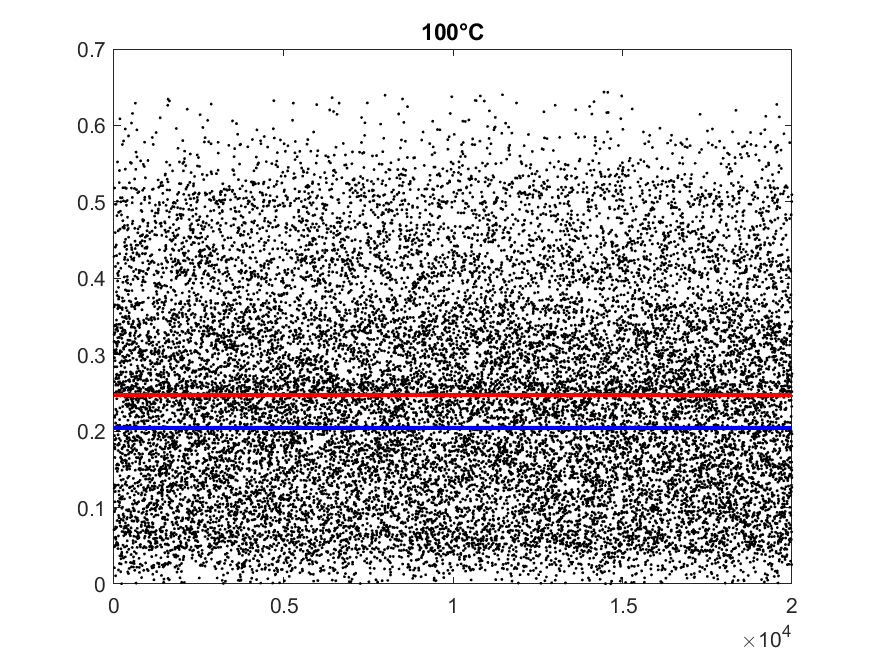
\includegraphics[width = 0.45\linewidth]{figures/histograph/scatter2.png}
	\end{subfigure}
	\begin{subfigure}{}
	\centering
	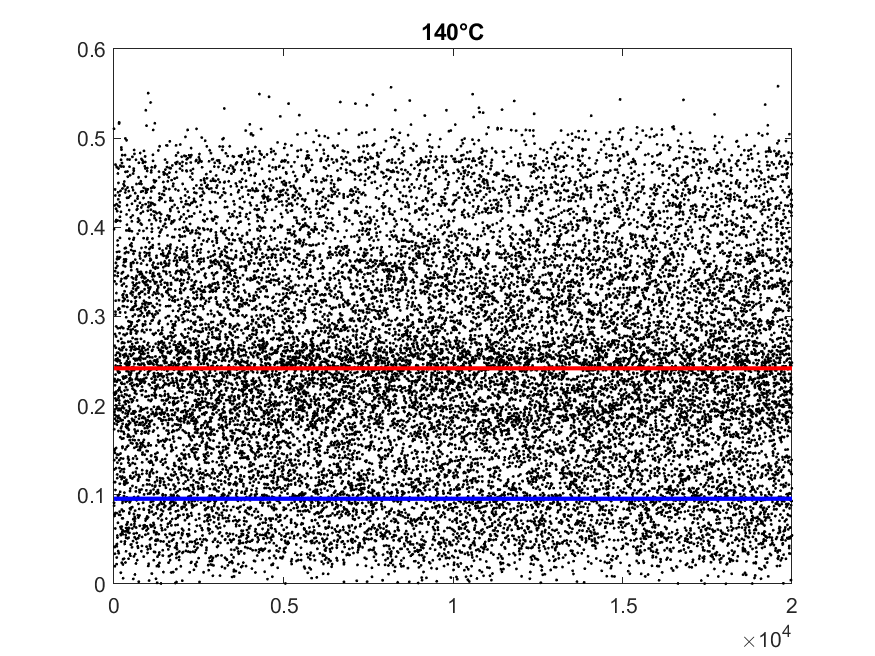
\includegraphics[width = 0.45\linewidth]{figures/histograph/scatter3.png}
	\end{subfigure}
	\begin{subfigure}{}
	\centering
	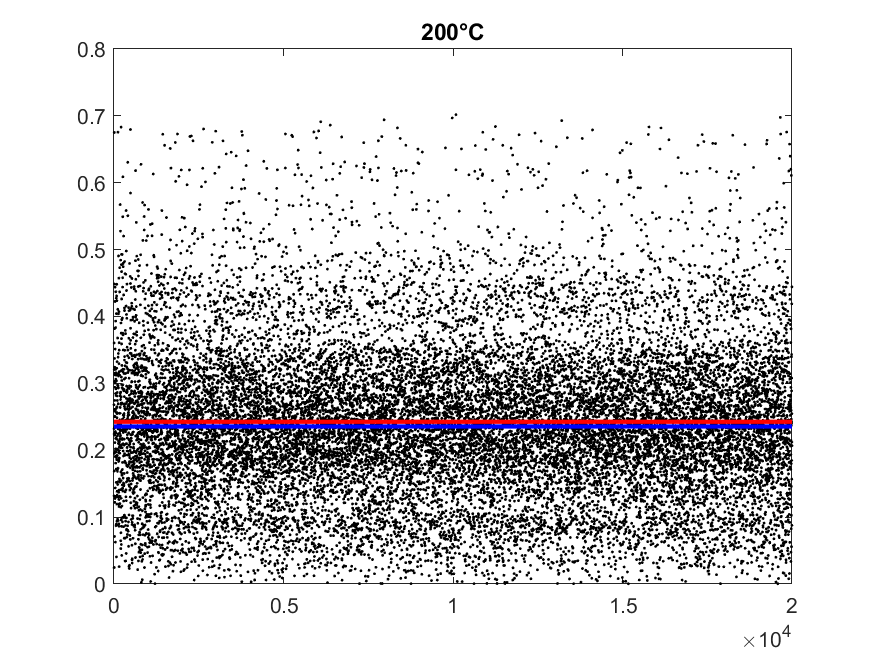
\includegraphics[width = 0.45\linewidth]{figures/histograph/scatter4.png}
	\end{subfigure}
	\begin{subfigure}{}
	\centering
	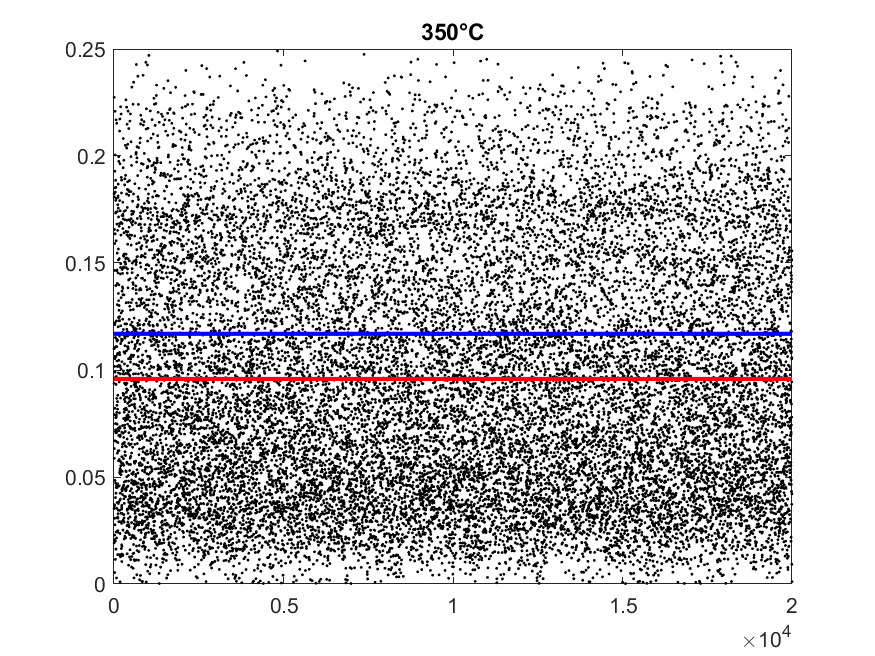
\includegraphics[width = 0.45\linewidth]{figures/histograph/scatter5.png}
	\end{subfigure}
	\begin{subfigure}{}
	\centering
	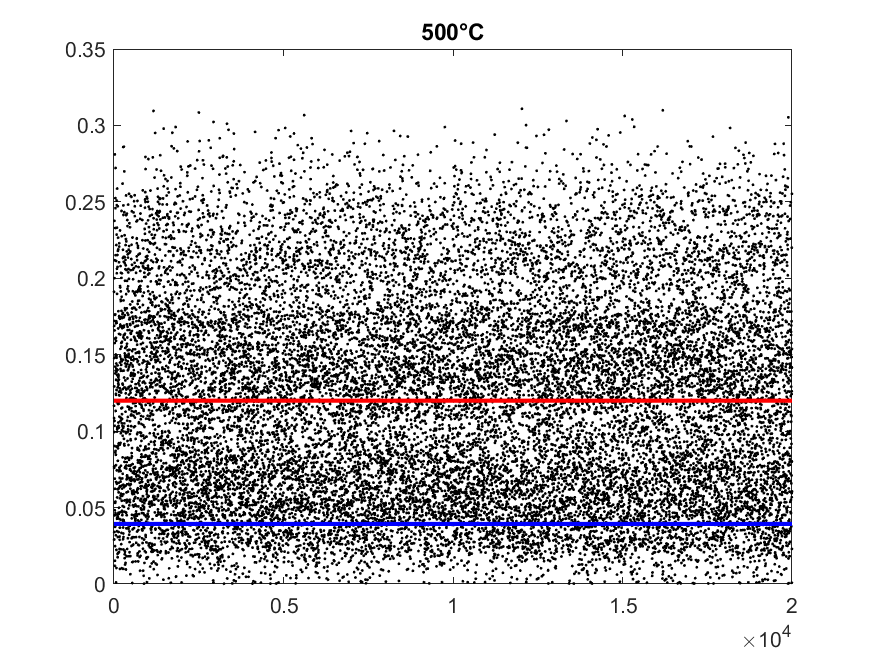
\includegraphics[width = 0.45\linewidth]{figures/histograph/scatter6.png}
	\end{subfigure}
	\begin{subfigure}{}
	\centering
	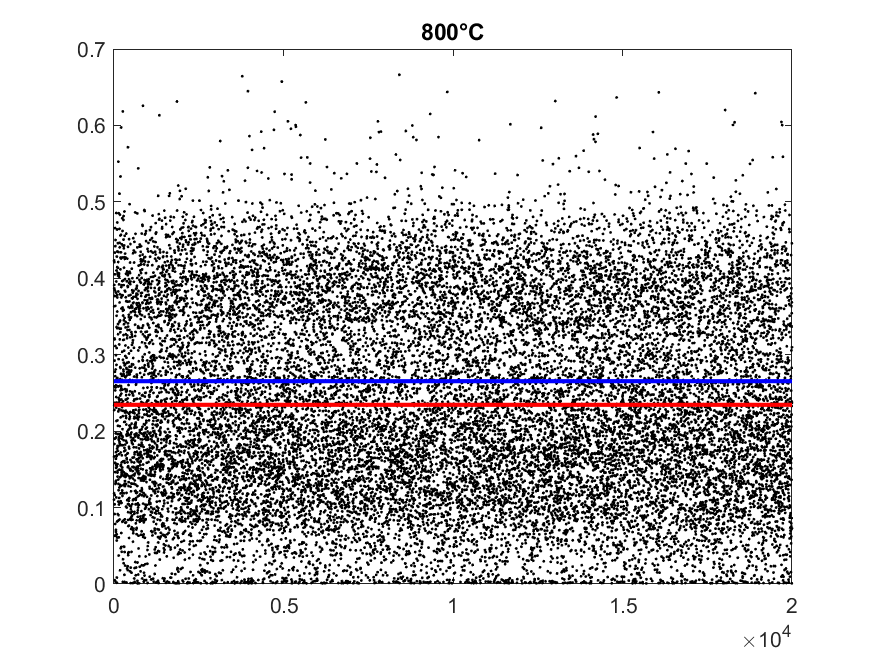
\includegraphics[width = 0.45\linewidth]{figures/histograph/scatter7.png}
	\end{subfigure}
	\begin{subfigure}{}
	\centering
	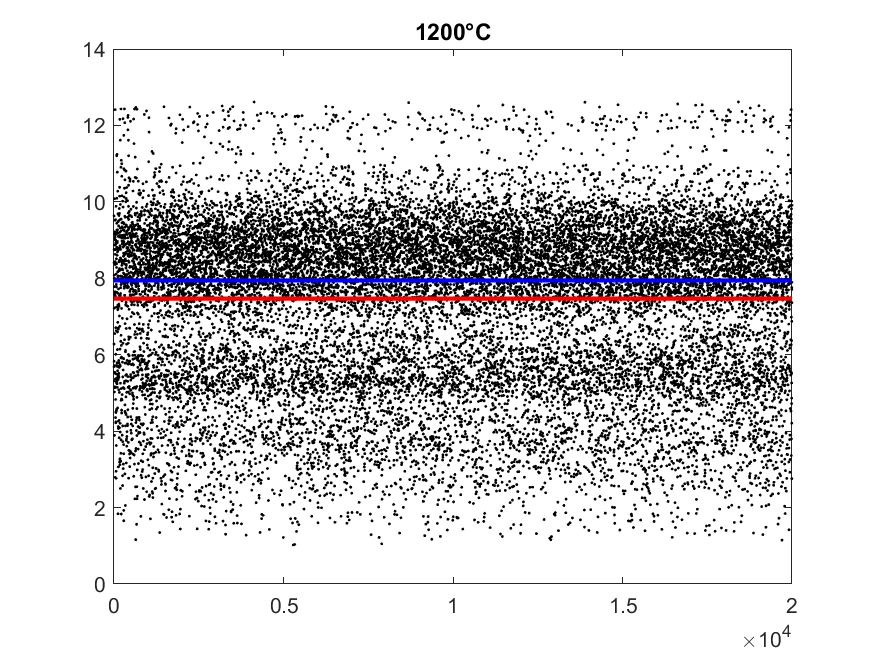
\includegraphics[width = 0.45\linewidth]{figures/histograph/scatter8.png}
	\end{subfigure}
	\centering
	\begin{subfigure}{}
	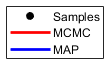
\includegraphics[width = 0.2\linewidth]{figures/histograph/scatter_legend.png}
	\end{subfigure}
	\caption{Distribution of samples at different temperatures with MCMC and MAP results indicated}
\end{figure}

\subsection{Evaluation of error}
Despite the uncertainties connected to the problem, a quantifiable measure of error is still required to allow unbiased assessment of the success of the algorithm and results.
The obtained $\kappa$-values will be used to rerun the model and obtain the new modelled temperature for each depth. 
For each depth the error will be quantified using the norm of the relative error at the seven different depths, denoted as $i$.
The relative error will be calculated according to  Equation \ref{relerror}. 
The new modelled output errors are compared to the Eurocode $\kappa$-value output errors to assess if the methods used produced a more accurate representation of the data.
The error at different depths are summarised in Table \ref{errortab} and the lowest error at that depth is highlighted in green. 
At a depth of 0mm none of the errors are highlighted as this temperature is independent of the $\kappa$-values.
This error measurement can be used to asses the error in the model or assumptions made to obtain the model.
It is important to note that this error does not only quantify the error in the thermal conductivity but any errors due to model assumptions are also encompassed.

\begin{equation}\label{relerror}
\epsilon _i = \frac{\norm{\hat{x}_i-x_i }_2}{\norm{x_i}_2} \quad \quad i= 1, ... ,7
\end{equation}

\begin{table}[H] 
\centering
\caption{Summary of error between models and data}
\label{errortab}
	\begin{tabular}{ r r r r }
	\toprule
	Depth(mm) & EURO & MAP & MCMC\\
	\midrule
	0 & 0.289 & 0.289 & 0.289\\
	16.5 & 0.217 & \cellcolor{green!20}0.194 & 0.205\\
	33 & 0.301   & \cellcolor{green!20} 0.191 & 0.200\\
	49.5 & 0.569 & 0.348 &\cellcolor{green!20} 0.323\\
	66 & 0.547   & 0.316 & \cellcolor{green!20}0.267\\
	82.5 & 0.501 &\cellcolor{green!20} 0.339 & 0.358\\
	99 & 0.219   & 0.219 &\cellcolor{green!20} 0.219\\
	\bottomrule	
	\end{tabular}
	
\end{table}

\subsection{Thermal diffusivity}
The main intent of this project was to determine the thermal diffusivity of SA-Pine. 
In Table \ref{diffrestab} the resulting thermal diffusivity is shown.
The thermal diffusivity was calculated using the information in Table \ref{cptab} and Equation \ref{alphaeq}.

\begin{table}[H]
\centering
	\caption{Resulting thermal diffusivity($\alpha \ten{-4}$)in m/s$^2$ }
	 \label{diffrestab}
	\begin{tabular}{ r r r r }
	\toprule
	Temp \textdegree C & EURO & MAP & MCMC\\
	\midrule
	0&   $1.64$&	$0.85$&	$1.64$\\
	60&  $1.64$&	$2.58$&	$3.79$\\
	100& $1.64$&	$2.78$&	$3.37$\\\
	140& $1.64$&	$1.31$&	$3.30$\\
	200& $2.05$&	$3.21$&	$3.32$\\
	350& $0.96$&	$1.60$&	$1.31$\\
	500& $1.23$&	$0.53$&	$1.64$\\
	800& $4.78$&	$3.62$&	$3.19$\\
	1200& $25.00$&	$108.00$&	$102.00$\\
	\bottomrule	
	\end{tabular}
	
\end{table}

\begin{sidewaysfigure}
	
	\centering
	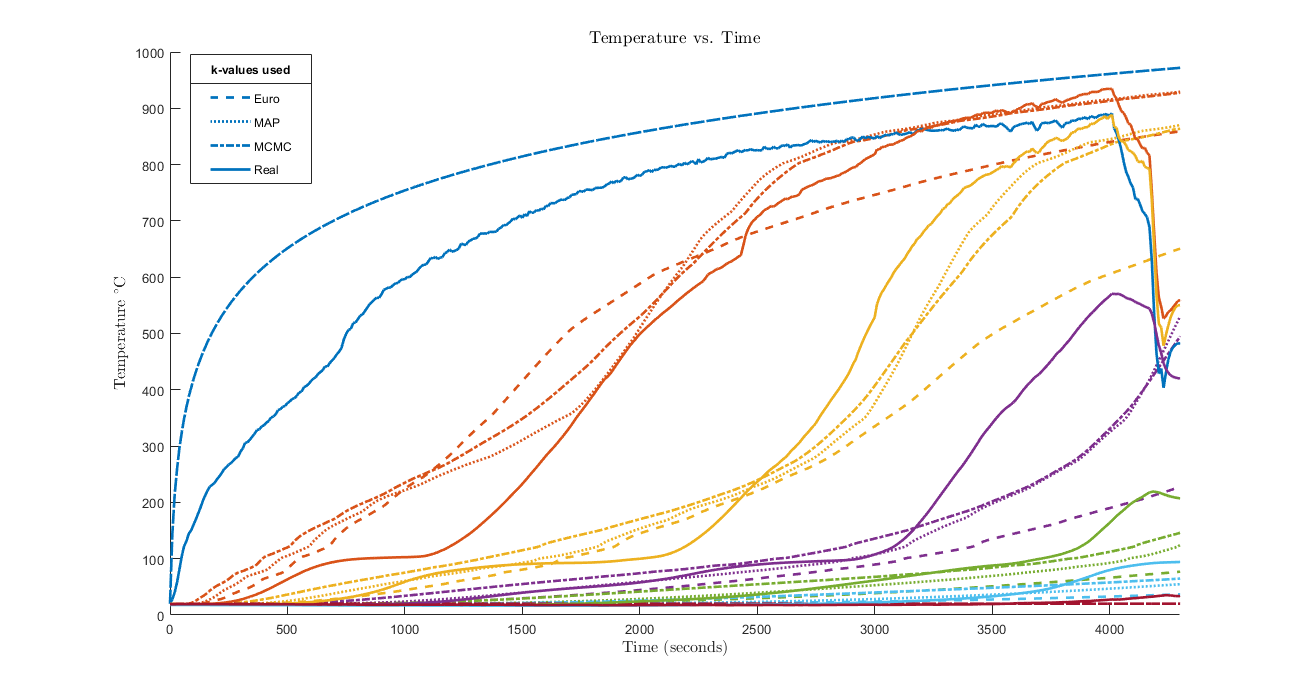
\includegraphics[width=\linewidth,]{figures/final_graph.png}
	\caption{Graph of measured data compared to model output}
	\label{final_graph}
\end{sidewaysfigure}






 \chapter{Discussion} \label{discussion}
 \chapter{Summary and Conclusion} \label{conclusion}

The usage of Markov Chain Monte-Carlo integration to solve for the thermal diffusivity of cross-laminated SA Pine was successful.
The adaptation of the finite element model derived from the heat conduction and diffusion equation enabled the creation of a posterior distribution.
The posterior distribution modelled after Bayes theory of inverse problems could be traversed and explored using the Markov Chain Monte-Carlo and the Maximum a Posteriori could be found using Nelder-Mead optimization.
The resulting $\kappa$ and $\alpha$ values produced a more accurate model of temperature over time.
There is a lot of potential for further optimization and fine-tuning of these algorithms and models.
With further development this concept could lead to simplified methods of calculating the fire rating of specifically SA-Pine as well as other timber samples.
More accurate and accessible fire ratings will help pave the way to improved fire safety.



\appendix%===========================================================
%
\chapter{Relevant code segments} \label{codeapp}
Below are the relevant code segments taken from the Matlab code that was used to generate the final samples used for analysis.

\section*{Prior function}
\begin{verbatim}
function q_val = prior_pdf(x_values,sigmaMU)

 global mu_values
 q_val = -0.5*((x_values - mu_values)*(x_values - mu_values)')/(sigmaMU^2);

end

\end{verbatim}
\chapter{Detailed results graph}
\begin{figure}
	\label{data_newk}
	\centering
	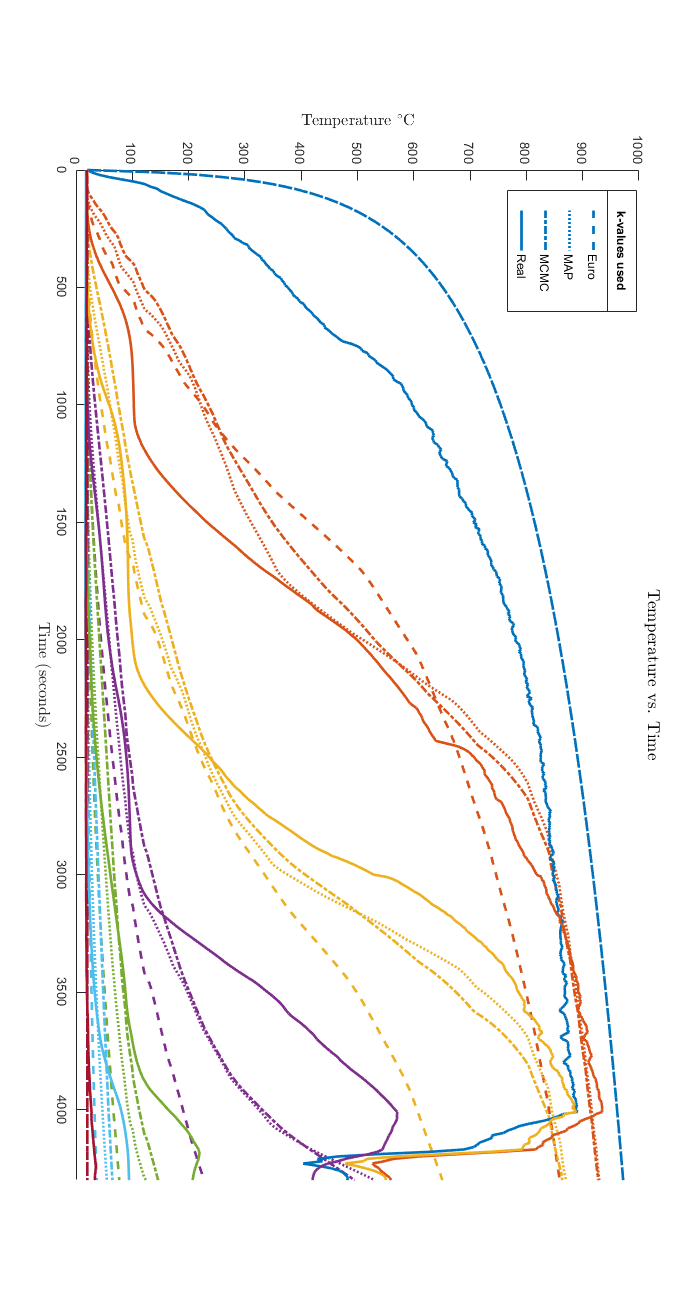
\includegraphics[width=0.8\linewidth,]{figures/final_graph_ver.png}
\end{figure}
\include{derive_app}
\include{Program}
\chapter{GA outcomes}



\backmatter%=========================================================

\bibliography{USBibsample}

\end{document}
